\documentclass[twoside]{book}

% Packages required by doxygen
\usepackage{fixltx2e}
\usepackage{calc}
\usepackage{doxygen}
\usepackage[export]{adjustbox} % also loads graphicx
\usepackage{graphicx}
\usepackage[utf8]{inputenc}
\usepackage{makeidx}
\usepackage{multicol}
\usepackage{multirow}
\PassOptionsToPackage{warn}{textcomp}
\usepackage{textcomp}
\usepackage[nointegrals]{wasysym}
\usepackage[table]{xcolor}

% Font selection
\usepackage[T1]{fontenc}
\usepackage[scaled=.90]{helvet}
\usepackage{courier}
\usepackage{amssymb}
\usepackage{sectsty}
\renewcommand{\familydefault}{\sfdefault}
\allsectionsfont{%
  \fontseries{bc}\selectfont%
  \color{darkgray}%
}
\renewcommand{\DoxyLabelFont}{%
  \fontseries{bc}\selectfont%
  \color{darkgray}%
}
\newcommand{\+}{\discretionary{\mbox{\scriptsize$\hookleftarrow$}}{}{}}

% Page & text layout
\usepackage{geometry}
\geometry{%
  a4paper,%
  top=2.5cm,%
  bottom=2.5cm,%
  left=2.5cm,%
  right=2.5cm%
}
\tolerance=750
\hfuzz=15pt
\hbadness=750
\setlength{\emergencystretch}{15pt}
\setlength{\parindent}{0cm}
\setlength{\parskip}{3ex plus 2ex minus 2ex}
\makeatletter
\renewcommand{\paragraph}{%
  \@startsection{paragraph}{4}{0ex}{-1.0ex}{1.0ex}{%
    \normalfont\normalsize\bfseries\SS@parafont%
  }%
}
\renewcommand{\subparagraph}{%
  \@startsection{subparagraph}{5}{0ex}{-1.0ex}{1.0ex}{%
    \normalfont\normalsize\bfseries\SS@subparafont%
  }%
}
\makeatother

% Headers & footers
\usepackage{fancyhdr}
\pagestyle{fancyplain}
\fancyhead[LE]{\fancyplain{}{\bfseries\thepage}}
\fancyhead[CE]{\fancyplain{}{}}
\fancyhead[RE]{\fancyplain{}{\bfseries\leftmark}}
\fancyhead[LO]{\fancyplain{}{\bfseries\rightmark}}
\fancyhead[CO]{\fancyplain{}{}}
\fancyhead[RO]{\fancyplain{}{\bfseries\thepage}}
\fancyfoot[LE]{\fancyplain{}{}}
\fancyfoot[CE]{\fancyplain{}{}}
\fancyfoot[RE]{\fancyplain{}{\bfseries\scriptsize Generated by Doxygen }}
\fancyfoot[LO]{\fancyplain{}{\bfseries\scriptsize Generated by Doxygen }}
\fancyfoot[CO]{\fancyplain{}{}}
\fancyfoot[RO]{\fancyplain{}{}}
\renewcommand{\footrulewidth}{0.4pt}
\renewcommand{\chaptermark}[1]{%
  \markboth{#1}{}%
}
\renewcommand{\sectionmark}[1]{%
  \markright{\thesection\ #1}%
}

% Indices & bibliography
\usepackage{natbib}
\usepackage[titles]{tocloft}
\setcounter{tocdepth}{3}
\setcounter{secnumdepth}{5}
\makeindex

% Hyperlinks (required, but should be loaded last)
\usepackage{ifpdf}
\ifpdf
  \usepackage[pdftex,pagebackref=true]{hyperref}
\else
  \usepackage[ps2pdf,pagebackref=true]{hyperref}
\fi
\hypersetup{%
  colorlinks=true,%
  linkcolor=blue,%
  citecolor=blue,%
  unicode%
}

% Custom commands
\newcommand{\clearemptydoublepage}{%
  \newpage{\pagestyle{empty}\cleardoublepage}%
}

\usepackage{caption}
\captionsetup{labelsep=space,justification=centering,font={bf},singlelinecheck=off,skip=4pt,position=top}

%===== C O N T E N T S =====

\begin{document}

% Titlepage & ToC
\hypersetup{pageanchor=false,
             bookmarksnumbered=true,
             pdfencoding=unicode
            }
\pagenumbering{roman}
\begin{titlepage}
\vspace*{7cm}
\begin{center}%
{\Large j-\/pet-\/ortho-\/simulations \\[1ex]\large 1.\+2 }\\
\vspace*{1cm}
{\large Generated by Doxygen 1.8.11}\\
\end{center}
\end{titlepage}
\clearemptydoublepage
\tableofcontents
\clearemptydoublepage
\pagenumbering{arabic}
\hypersetup{pageanchor=true}

%--- Begin generated contents ---
\chapter{Class Index}
\section{Class List}
Here are the classes, structs, unions and interfaces with brief descriptions\+:\begin{DoxyCompactList}
\item\contentsline{section}{\hyperlink{classComptonScattering}{Compton\+Scattering} \\*Class responsible for Compton scattering according to the Klein-\/\+Nishina formula }{\pageref{classComptonScattering}}{}
\item\contentsline{section}{\hyperlink{classParamManager}{Param\+Manager} \\*Class responsible for loadind simulation parameters from external file. (by default simulation\+\_\+parameters.\+par) }{\pageref{classParamManager}}{}
\item\contentsline{section}{\hyperlink{classPsDecay}{Ps\+Decay} \\*Contains histograms with gammas\textquotesingle{} characteristics and inforamtion about passed cuts. }{\pageref{classPsDecay}}{}
\end{DoxyCompactList}

\chapter{File Index}
\section{File List}
Here is a list of all files with brief descriptions\+:\begin{DoxyCompactList}
\item\contentsline{section}{/home/rafal/\+Projekty/j-\/pet-\/ortho-\/simulations/src/\hyperlink{comptonscattering_8cpp}{comptonscattering.\+cpp} }{\pageref{comptonscattering_8cpp}}{}
\item\contentsline{section}{/home/rafal/\+Projekty/j-\/pet-\/ortho-\/simulations/src/\hyperlink{comptonscattering_8h}{comptonscattering.\+h} }{\pageref{comptonscattering_8h}}{}
\item\contentsline{section}{/home/rafal/\+Projekty/j-\/pet-\/ortho-\/simulations/src/\hyperlink{constants_8h}{constants.\+h} }{\pageref{constants_8h}}{}
\item\contentsline{section}{/home/rafal/\+Projekty/j-\/pet-\/ortho-\/simulations/src/\hyperlink{parammanager_8cpp}{parammanager.\+cpp} }{\pageref{parammanager_8cpp}}{}
\item\contentsline{section}{/home/rafal/\+Projekty/j-\/pet-\/ortho-\/simulations/src/\hyperlink{parammanager_8h}{parammanager.\+h} }{\pageref{parammanager_8h}}{}
\item\contentsline{section}{/home/rafal/\+Projekty/j-\/pet-\/ortho-\/simulations/src/\hyperlink{psdecay_8cpp}{psdecay.\+cpp} }{\pageref{psdecay_8cpp}}{}
\item\contentsline{section}{/home/rafal/\+Projekty/j-\/pet-\/ortho-\/simulations/src/\hyperlink{psdecay_8h}{psdecay.\+h} }{\pageref{psdecay_8h}}{}
\item\contentsline{section}{/home/rafal/\+Projekty/j-\/pet-\/ortho-\/simulations/src/\hyperlink{simulate_8cpp}{simulate.\+cpp} }{\pageref{simulate_8cpp}}{}
\end{DoxyCompactList}

\chapter{Class Documentation}
\hypertarget{classComptonScattering}{}\section{Compton\+Scattering Class Reference}
\label{classComptonScattering}\index{Compton\+Scattering@{Compton\+Scattering}}


The \hyperlink{classComptonScattering}{Compton\+Scattering} class Class responsible for Compton scattering according to the Klein-\/\+Nishina formula.  




{\ttfamily \#include $<$comptonscattering.\+h$>$}

\subsection*{Public Member Functions}
\begin{DoxyCompactItemize}
\item 
\hyperlink{classComptonScattering_a3c50437f33ee40fcab617676ae36bb6b}{Compton\+Scattering} (int no\+Of\+Gammas=0)
\begin{DoxyCompactList}\small\item\em \hyperlink{classComptonScattering_a3c50437f33ee40fcab617676ae36bb6b}{Compton\+Scattering\+::\+Compton\+Scattering} Basic constructor. \end{DoxyCompactList}\item 
\hyperlink{classComptonScattering_a09713fba1b6ef5e3f8bd11253336e0b1}{Compton\+Scattering} (const \hyperlink{classComptonScattering}{Compton\+Scattering} \&est)
\begin{DoxyCompactList}\small\item\em \hyperlink{classComptonScattering_a3c50437f33ee40fcab617676ae36bb6b}{Compton\+Scattering\+::\+Compton\+Scattering} Copy constructor. \end{DoxyCompactList}\item 
\hyperlink{classComptonScattering}{Compton\+Scattering} \& \hyperlink{classComptonScattering_af450ec96e7bd187249b4d9693342e262}{operator=} (const \hyperlink{classComptonScattering}{Compton\+Scattering} \&est)
\begin{DoxyCompactList}\small\item\em \hyperlink{classComptonScattering_af450ec96e7bd187249b4d9693342e262}{Compton\+Scattering\+::operator =} Copies histograms and field values. \end{DoxyCompactList}\item 
\hyperlink{classComptonScattering_a949a87ad889d53ea2cb2e1597ccf9c55}{$\sim$\+Compton\+Scattering} ()
\begin{DoxyCompactList}\small\item\em \hyperlink{classComptonScattering_a949a87ad889d53ea2cb2e1597ccf9c55}{Compton\+Scattering\+::$\sim$\+Compton\+Scattering} Destructor, releases memory after histograms. \end{DoxyCompactList}\item 
void \hyperlink{classComptonScattering_a1da6f97e6702c6a49b6527b73d59d6c8}{Draw\+P\+DF} (std\+::string file\+Prefix=\char`\"{}\char`\"{})
\begin{DoxyCompactList}\small\item\em \hyperlink{classComptonScattering_a1da6f97e6702c6a49b6527b73d59d6c8}{Compton\+Scattering\+::\+Draw\+P\+DF} Draws Klein-\/\+Nishina function and saves to a file. \end{DoxyCompactList}\item 
void \hyperlink{classComptonScattering_ae04a6b8cc58e6b9c5455e0a38d42330d}{Draw\+Electron\+Dist} (std\+::string file\+Prefix=\char`\"{}\char`\"{})
\begin{DoxyCompactList}\small\item\em \hyperlink{classComptonScattering_ae04a6b8cc58e6b9c5455e0a38d42330d}{Compton\+Scattering\+::\+Draw\+Electron\+Dist} Draws and saves to file energy of Compton electrons and angle distributions for scattered photons. \end{DoxyCompactList}\item 
void \hyperlink{classComptonScattering_ada62d267585a2e3772d01b064e875756}{Scatter} (double E)
\begin{DoxyCompactList}\small\item\em \hyperlink{classComptonScattering_ada62d267585a2e3772d01b064e875756}{Compton\+Scattering\+::\+Scatter} Scatters a photon according to Klein-\/\+Nishina formula and fills histograms for electrons. \end{DoxyCompactList}\end{DoxyCompactItemize}
\subsection*{Public Attributes}
\begin{DoxyCompactItemize}
\item 
T\+F1 $\ast$ \hyperlink{classComptonScattering_add23479fa60d3dab59f9baa2d2dcf76f}{f\+P\+DF}
\end{DoxyCompactItemize}
\subsection*{Static Private Member Functions}
\begin{DoxyCompactItemize}
\item 
static long double \hyperlink{classComptonScattering_a0723eb40298a7697e6f3cbdb241eb19e}{Klein\+Nishina\+\_\+} (double $\ast$angle, double $\ast$energy)
\begin{DoxyCompactList}\small\item\em Compton\+Scattering\+::\+Klein\+Nishima Calculates P\+DF according to Klein Nishima formula. \end{DoxyCompactList}\end{DoxyCompactItemize}
\subsection*{Private Attributes}
\begin{DoxyCompactItemize}
\item 
int \hyperlink{classComptonScattering_a7a0703c812fb29b0c80c251ae70ce0e9}{f\+No\+Of\+Gammas\+\_\+}
\item 
T\+H1F $\ast$ \hyperlink{classComptonScattering_a27362e48e05442df8508d12d3492f130}{f\+H\+\_\+electron\+\_\+\+E\+\_\+}
\item 
T\+H1F $\ast$ \hyperlink{classComptonScattering_ac2f4da687eadc32b94a80fe82f8e5a2b}{f\+H\+\_\+photon\+\_\+theta\+\_\+}
\item 
T\+H2D $\ast$ \hyperlink{classComptonScattering_aecd1718d8d180ff66e3a89f297f4458d}{f\+H\+\_\+\+P\+D\+F\+\_\+}
\end{DoxyCompactItemize}


\subsection{Detailed Description}
The \hyperlink{classComptonScattering}{Compton\+Scattering} class Class responsible for Compton scattering according to the Klein-\/\+Nishina formula. 

\subsection{Constructor \& Destructor Documentation}
\index{Compton\+Scattering@{Compton\+Scattering}!Compton\+Scattering@{Compton\+Scattering}}
\index{Compton\+Scattering@{Compton\+Scattering}!Compton\+Scattering@{Compton\+Scattering}}
\subsubsection[{\texorpdfstring{Compton\+Scattering(int no\+Of\+Gammas=0)}{ComptonScattering(int noOfGammas=0)}}]{\setlength{\rightskip}{0pt plus 5cm}Compton\+Scattering\+::\+Compton\+Scattering (
\begin{DoxyParamCaption}
\item[{int}]{no\+Of\+Gammas = {\ttfamily 0}}
\end{DoxyParamCaption}
)}\hypertarget{classComptonScattering_a3c50437f33ee40fcab617676ae36bb6b}{}\label{classComptonScattering_a3c50437f33ee40fcab617676ae36bb6b}


\hyperlink{classComptonScattering_a3c50437f33ee40fcab617676ae36bb6b}{Compton\+Scattering\+::\+Compton\+Scattering} Basic constructor. 


\begin{DoxyParams}{Parameters}
{\em prefix} & File prefix. \\
\hline
{\em no\+Of\+Gammas} & No of gammas (only for file naming). \\
\hline
\end{DoxyParams}
\index{Compton\+Scattering@{Compton\+Scattering}!Compton\+Scattering@{Compton\+Scattering}}
\index{Compton\+Scattering@{Compton\+Scattering}!Compton\+Scattering@{Compton\+Scattering}}
\subsubsection[{\texorpdfstring{Compton\+Scattering(const Compton\+Scattering \&est)}{ComptonScattering(const ComptonScattering &est)}}]{\setlength{\rightskip}{0pt plus 5cm}Compton\+Scattering\+::\+Compton\+Scattering (
\begin{DoxyParamCaption}
\item[{const {\bf Compton\+Scattering} \&}]{est}
\end{DoxyParamCaption}
)}\hypertarget{classComptonScattering_a09713fba1b6ef5e3f8bd11253336e0b1}{}\label{classComptonScattering_a09713fba1b6ef5e3f8bd11253336e0b1}


\hyperlink{classComptonScattering_a3c50437f33ee40fcab617676ae36bb6b}{Compton\+Scattering\+::\+Compton\+Scattering} Copy constructor. 


\begin{DoxyParams}{Parameters}
{\em est} & \hyperlink{classComptonScattering}{Compton\+Scattering} instance to be copied. \\
\hline
\end{DoxyParams}
\index{Compton\+Scattering@{Compton\+Scattering}!````~Compton\+Scattering@{$\sim$\+Compton\+Scattering}}
\index{````~Compton\+Scattering@{$\sim$\+Compton\+Scattering}!Compton\+Scattering@{Compton\+Scattering}}
\subsubsection[{\texorpdfstring{$\sim$\+Compton\+Scattering()}{~ComptonScattering()}}]{\setlength{\rightskip}{0pt plus 5cm}Compton\+Scattering\+::$\sim$\+Compton\+Scattering (
\begin{DoxyParamCaption}
{}
\end{DoxyParamCaption}
)}\hypertarget{classComptonScattering_a949a87ad889d53ea2cb2e1597ccf9c55}{}\label{classComptonScattering_a949a87ad889d53ea2cb2e1597ccf9c55}


\hyperlink{classComptonScattering_a949a87ad889d53ea2cb2e1597ccf9c55}{Compton\+Scattering\+::$\sim$\+Compton\+Scattering} Destructor, releases memory after histograms. 



\subsection{Member Function Documentation}
\index{Compton\+Scattering@{Compton\+Scattering}!Draw\+Electron\+Dist@{Draw\+Electron\+Dist}}
\index{Draw\+Electron\+Dist@{Draw\+Electron\+Dist}!Compton\+Scattering@{Compton\+Scattering}}
\subsubsection[{\texorpdfstring{Draw\+Electron\+Dist(std\+::string file\+Prefix="""")}{DrawElectronDist(std::string filePrefix="")}}]{\setlength{\rightskip}{0pt plus 5cm}void Compton\+Scattering\+::\+Draw\+Electron\+Dist (
\begin{DoxyParamCaption}
\item[{std\+::string}]{file\+Prefix = {\ttfamily \char`\"{}\char`\"{}}}
\end{DoxyParamCaption}
)}\hypertarget{classComptonScattering_ae04a6b8cc58e6b9c5455e0a38d42330d}{}\label{classComptonScattering_ae04a6b8cc58e6b9c5455e0a38d42330d}


\hyperlink{classComptonScattering_ae04a6b8cc58e6b9c5455e0a38d42330d}{Compton\+Scattering\+::\+Draw\+Electron\+Dist} Draws and saves to file energy of Compton electrons and angle distributions for scattered photons. 


\begin{DoxyParams}{Parameters}
{\em file\+Prefix} & Prefix of the output file, may contain path. \\
\hline
\end{DoxyParams}
\index{Compton\+Scattering@{Compton\+Scattering}!Draw\+P\+DF@{Draw\+P\+DF}}
\index{Draw\+P\+DF@{Draw\+P\+DF}!Compton\+Scattering@{Compton\+Scattering}}
\subsubsection[{\texorpdfstring{Draw\+P\+D\+F(std\+::string file\+Prefix="""")}{DrawPDF(std::string filePrefix="")}}]{\setlength{\rightskip}{0pt plus 5cm}void Compton\+Scattering\+::\+Draw\+P\+DF (
\begin{DoxyParamCaption}
\item[{std\+::string}]{file\+Prefix = {\ttfamily \char`\"{}\char`\"{}}}
\end{DoxyParamCaption}
)}\hypertarget{classComptonScattering_a1da6f97e6702c6a49b6527b73d59d6c8}{}\label{classComptonScattering_a1da6f97e6702c6a49b6527b73d59d6c8}


\hyperlink{classComptonScattering_a1da6f97e6702c6a49b6527b73d59d6c8}{Compton\+Scattering\+::\+Draw\+P\+DF} Draws Klein-\/\+Nishina function and saves to a file. 


\begin{DoxyParams}{Parameters}
{\em file\+Prefix} & Prefix of the output file, may contain path. \\
\hline
\end{DoxyParams}
\index{Compton\+Scattering@{Compton\+Scattering}!Klein\+Nishina\+\_\+@{Klein\+Nishina\+\_\+}}
\index{Klein\+Nishina\+\_\+@{Klein\+Nishina\+\_\+}!Compton\+Scattering@{Compton\+Scattering}}
\subsubsection[{\texorpdfstring{Klein\+Nishina\+\_\+(double $\ast$angle, double $\ast$energy)}{KleinNishina_(double *angle, double *energy)}}]{\setlength{\rightskip}{0pt plus 5cm}long double Compton\+Scattering\+::\+Klein\+Nishina\+\_\+ (
\begin{DoxyParamCaption}
\item[{double $\ast$}]{angle, }
\item[{double $\ast$}]{energy}
\end{DoxyParamCaption}
)\hspace{0.3cm}{\ttfamily [static]}, {\ttfamily [private]}}\hypertarget{classComptonScattering_a0723eb40298a7697e6f3cbdb241eb19e}{}\label{classComptonScattering_a0723eb40298a7697e6f3cbdb241eb19e}


Compton\+Scattering\+::\+Klein\+Nishima Calculates P\+DF according to Klein Nishima formula. 


\begin{DoxyParams}{Parameters}
{\em x} & Array of values, x\mbox{[}0\mbox{]} -- incident photon\textquotesingle{}s energy, x\mbox{[}1\mbox{]} -- scattering angle \\
\hline
{\em params} & \\
\hline
\end{DoxyParams}
\begin{DoxyReturn}{Returns}
Value of the function. 
\end{DoxyReturn}
\index{Compton\+Scattering@{Compton\+Scattering}!operator=@{operator=}}
\index{operator=@{operator=}!Compton\+Scattering@{Compton\+Scattering}}
\subsubsection[{\texorpdfstring{operator=(const Compton\+Scattering \&est)}{operator=(const ComptonScattering &est)}}]{\setlength{\rightskip}{0pt plus 5cm}{\bf Compton\+Scattering} \& Compton\+Scattering\+::operator= (
\begin{DoxyParamCaption}
\item[{const {\bf Compton\+Scattering} \&}]{est}
\end{DoxyParamCaption}
)}\hypertarget{classComptonScattering_af450ec96e7bd187249b4d9693342e262}{}\label{classComptonScattering_af450ec96e7bd187249b4d9693342e262}


\hyperlink{classComptonScattering_af450ec96e7bd187249b4d9693342e262}{Compton\+Scattering\+::operator =} Copies histograms and field values. 


\begin{DoxyParams}{Parameters}
{\em est} & \hyperlink{classComptonScattering}{Compton\+Scattering} instance to be copied. \\
\hline
\end{DoxyParams}
\begin{DoxyReturn}{Returns}
Reference to \hyperlink{classComptonScattering}{Compton\+Scattering} instance with copied fields. 
\end{DoxyReturn}
\index{Compton\+Scattering@{Compton\+Scattering}!Scatter@{Scatter}}
\index{Scatter@{Scatter}!Compton\+Scattering@{Compton\+Scattering}}
\subsubsection[{\texorpdfstring{Scatter(double E)}{Scatter(double E)}}]{\setlength{\rightskip}{0pt plus 5cm}void Compton\+Scattering\+::\+Scatter (
\begin{DoxyParamCaption}
\item[{double}]{E}
\end{DoxyParamCaption}
)}\hypertarget{classComptonScattering_ada62d267585a2e3772d01b064e875756}{}\label{classComptonScattering_ada62d267585a2e3772d01b064e875756}


\hyperlink{classComptonScattering_ada62d267585a2e3772d01b064e875756}{Compton\+Scattering\+::\+Scatter} Scatters a photon according to Klein-\/\+Nishina formula and fills histograms for electrons. 


\begin{DoxyParams}{Parameters}
{\em E} & Energy of incident photon. \\
\hline
\end{DoxyParams}


\subsection{Member Data Documentation}
\index{Compton\+Scattering@{Compton\+Scattering}!f\+H\+\_\+electron\+\_\+\+E\+\_\+@{f\+H\+\_\+electron\+\_\+\+E\+\_\+}}
\index{f\+H\+\_\+electron\+\_\+\+E\+\_\+@{f\+H\+\_\+electron\+\_\+\+E\+\_\+}!Compton\+Scattering@{Compton\+Scattering}}
\subsubsection[{\texorpdfstring{f\+H\+\_\+electron\+\_\+\+E\+\_\+}{fH_electron_E_}}]{\setlength{\rightskip}{0pt plus 5cm}T\+H1F$\ast$ Compton\+Scattering\+::f\+H\+\_\+electron\+\_\+\+E\+\_\+\hspace{0.3cm}{\ttfamily [private]}}\hypertarget{classComptonScattering_a27362e48e05442df8508d12d3492f130}{}\label{classComptonScattering_a27362e48e05442df8508d12d3492f130}
\index{Compton\+Scattering@{Compton\+Scattering}!f\+H\+\_\+\+P\+D\+F\+\_\+@{f\+H\+\_\+\+P\+D\+F\+\_\+}}
\index{f\+H\+\_\+\+P\+D\+F\+\_\+@{f\+H\+\_\+\+P\+D\+F\+\_\+}!Compton\+Scattering@{Compton\+Scattering}}
\subsubsection[{\texorpdfstring{f\+H\+\_\+\+P\+D\+F\+\_\+}{fH_PDF_}}]{\setlength{\rightskip}{0pt plus 5cm}T\+H2D$\ast$ Compton\+Scattering\+::f\+H\+\_\+\+P\+D\+F\+\_\+\hspace{0.3cm}{\ttfamily [private]}}\hypertarget{classComptonScattering_aecd1718d8d180ff66e3a89f297f4458d}{}\label{classComptonScattering_aecd1718d8d180ff66e3a89f297f4458d}
\index{Compton\+Scattering@{Compton\+Scattering}!f\+H\+\_\+photon\+\_\+theta\+\_\+@{f\+H\+\_\+photon\+\_\+theta\+\_\+}}
\index{f\+H\+\_\+photon\+\_\+theta\+\_\+@{f\+H\+\_\+photon\+\_\+theta\+\_\+}!Compton\+Scattering@{Compton\+Scattering}}
\subsubsection[{\texorpdfstring{f\+H\+\_\+photon\+\_\+theta\+\_\+}{fH_photon_theta_}}]{\setlength{\rightskip}{0pt plus 5cm}T\+H1F$\ast$ Compton\+Scattering\+::f\+H\+\_\+photon\+\_\+theta\+\_\+\hspace{0.3cm}{\ttfamily [private]}}\hypertarget{classComptonScattering_ac2f4da687eadc32b94a80fe82f8e5a2b}{}\label{classComptonScattering_ac2f4da687eadc32b94a80fe82f8e5a2b}
\index{Compton\+Scattering@{Compton\+Scattering}!f\+No\+Of\+Gammas\+\_\+@{f\+No\+Of\+Gammas\+\_\+}}
\index{f\+No\+Of\+Gammas\+\_\+@{f\+No\+Of\+Gammas\+\_\+}!Compton\+Scattering@{Compton\+Scattering}}
\subsubsection[{\texorpdfstring{f\+No\+Of\+Gammas\+\_\+}{fNoOfGammas_}}]{\setlength{\rightskip}{0pt plus 5cm}int Compton\+Scattering\+::f\+No\+Of\+Gammas\+\_\+\hspace{0.3cm}{\ttfamily [private]}}\hypertarget{classComptonScattering_a7a0703c812fb29b0c80c251ae70ce0e9}{}\label{classComptonScattering_a7a0703c812fb29b0c80c251ae70ce0e9}
\index{Compton\+Scattering@{Compton\+Scattering}!f\+P\+DF@{f\+P\+DF}}
\index{f\+P\+DF@{f\+P\+DF}!Compton\+Scattering@{Compton\+Scattering}}
\subsubsection[{\texorpdfstring{f\+P\+DF}{fPDF}}]{\setlength{\rightskip}{0pt plus 5cm}T\+F1$\ast$ Compton\+Scattering\+::f\+P\+DF}\hypertarget{classComptonScattering_add23479fa60d3dab59f9baa2d2dcf76f}{}\label{classComptonScattering_add23479fa60d3dab59f9baa2d2dcf76f}


The documentation for this class was generated from the following files\+:\begin{DoxyCompactItemize}
\item 
src/\hyperlink{comptonscattering_8h}{comptonscattering.\+h}\item 
src/\hyperlink{comptonscattering_8cpp}{comptonscattering.\+cpp}\end{DoxyCompactItemize}

\hypertarget{classParamManager}{}\section{Param\+Manager Class Reference}
\label{classParamManager}\index{Param\+Manager@{Param\+Manager}}


The \hyperlink{classParamManager}{Param\+Manager} class Class responsible for loadind simulation parameters from external file. (by default simulation\+\_\+parameters.\+par)  




{\ttfamily \#include $<$parammanager.\+h$>$}

\subsection*{Public Member Functions}
\begin{DoxyCompactItemize}
\item 
\hyperlink{classParamManager_a2950d2af06c631b83e0d723765dcacfa}{Param\+Manager} ()
\begin{DoxyCompactList}\small\item\em \hyperlink{classParamManager_a2950d2af06c631b83e0d723765dcacfa}{Param\+Manager\+::\+Param\+Manager} Basic constructor. \end{DoxyCompactList}\item 
\hyperlink{classParamManager_a6f0dcb6c03fbacea1fdd78d1410ad776}{Param\+Manager} (const \hyperlink{classParamManager}{Param\+Manager} \&pm)
\begin{DoxyCompactList}\small\item\em \hyperlink{classParamManager_a2950d2af06c631b83e0d723765dcacfa}{Param\+Manager\+::\+Param\+Manager} Copy constructor. \end{DoxyCompactList}\item 
\hyperlink{classParamManager}{Param\+Manager} \& \hyperlink{classParamManager_ae4e63f59a1352a3602cb464ab24ef623}{operator=} (const \hyperlink{classParamManager}{Param\+Manager} \&est)
\begin{DoxyCompactList}\small\item\em \hyperlink{classParamManager_ae4e63f59a1352a3602cb464ab24ef623}{Param\+Manager\+::operator =} Assignement operator. \end{DoxyCompactList}\item 
double \hyperlink{classParamManager_ae58712c5696b4922b86048725b8c4501}{get\+Sim\+Steps} ()
\item 
double \hyperlink{classParamManager_ae02f327dc44c89493a8715f0d943b816}{get\+Sim\+Runs} ()
\item 
std\+::vector$<$ double $>$ \hyperlink{classParamManager_a9922b859162ad477b908c4251e90ca99}{get\+Data\+At} (int index=0)
\begin{DoxyCompactList}\small\item\em \hyperlink{classParamManager_a9922b859162ad477b908c4251e90ca99}{Param\+Manager\+::get\+Data\+At} Used to get source\textquotesingle{}s position and momentum. \end{DoxyCompactList}\item 
void \hyperlink{classParamManager_a8708a6a6ab26ceb69d856996f2f9085f}{Import\+Params} (std\+::string in\+File=\char`\"{}simulation\+\_\+parameters.\+par\char`\"{})
\begin{DoxyCompactList}\small\item\em \hyperlink{classParamManager_a8708a6a6ab26ceb69d856996f2f9085f}{Param\+Manager\+::\+Import\+Params} Imports prameters from file. It reads the number of simulation steps from the first line, and source\textquotesingle{}s (x,y,z,px,py,pz) from the nect ones. \end{DoxyCompactList}\item 
bool \hyperlink{classParamManager_abcaeb584edbc8949339f3a71f0cae3ce}{operator==} (const \hyperlink{classParamManager}{Param\+Manager} \&pm) const 
\begin{DoxyCompactList}\small\item\em \hyperlink{classParamManager_abcaeb584edbc8949339f3a71f0cae3ce}{Param\+Manager\+::operator ==} Compare operator. Compares values of member fields. \end{DoxyCompactList}\end{DoxyCompactItemize}
\subsection*{Private Attributes}
\begin{DoxyCompactItemize}
\item 
int \hyperlink{classParamManager_a6020a91cb4adc8f9dcd6647353840599}{f\+Sim\+Steps\+\_\+}
\item 
int \hyperlink{classParamManager_a3f867447d92ddea2da69014308ad0d16}{f\+Sim\+Runs\+\_\+}
\item 
std\+::vector$<$ std\+::vector$<$ double $>$ $>$ \hyperlink{classParamManager_a50cc8e69bb08c7f0b32d7614d5ade323}{f\+Data\+\_\+}
\end{DoxyCompactItemize}


\subsection{Detailed Description}
The \hyperlink{classParamManager}{Param\+Manager} class Class responsible for loadind simulation parameters from external file. (by default simulation\+\_\+parameters.\+par) 

\subsection{Constructor \& Destructor Documentation}
\index{Param\+Manager@{Param\+Manager}!Param\+Manager@{Param\+Manager}}
\index{Param\+Manager@{Param\+Manager}!Param\+Manager@{Param\+Manager}}
\subsubsection[{\texorpdfstring{Param\+Manager()}{ParamManager()}}]{\setlength{\rightskip}{0pt plus 5cm}Param\+Manager\+::\+Param\+Manager (
\begin{DoxyParamCaption}
{}
\end{DoxyParamCaption}
)}\hypertarget{classParamManager_a2950d2af06c631b83e0d723765dcacfa}{}\label{classParamManager_a2950d2af06c631b83e0d723765dcacfa}


\hyperlink{classParamManager_a2950d2af06c631b83e0d723765dcacfa}{Param\+Manager\+::\+Param\+Manager} Basic constructor. 

\index{Param\+Manager@{Param\+Manager}!Param\+Manager@{Param\+Manager}}
\index{Param\+Manager@{Param\+Manager}!Param\+Manager@{Param\+Manager}}
\subsubsection[{\texorpdfstring{Param\+Manager(const Param\+Manager \&pm)}{ParamManager(const ParamManager &pm)}}]{\setlength{\rightskip}{0pt plus 5cm}Param\+Manager\+::\+Param\+Manager (
\begin{DoxyParamCaption}
\item[{const {\bf Param\+Manager} \&}]{est}
\end{DoxyParamCaption}
)}\hypertarget{classParamManager_a6f0dcb6c03fbacea1fdd78d1410ad776}{}\label{classParamManager_a6f0dcb6c03fbacea1fdd78d1410ad776}


\hyperlink{classParamManager_a2950d2af06c631b83e0d723765dcacfa}{Param\+Manager\+::\+Param\+Manager} Copy constructor. 


\begin{DoxyParams}{Parameters}
{\em est} & \hyperlink{classParamManager}{Param\+Manager} instance from which fields will be copied. \\
\hline
\end{DoxyParams}


\subsection{Member Function Documentation}
\index{Param\+Manager@{Param\+Manager}!get\+Data\+At@{get\+Data\+At}}
\index{get\+Data\+At@{get\+Data\+At}!Param\+Manager@{Param\+Manager}}
\subsubsection[{\texorpdfstring{get\+Data\+At(int index=0)}{getDataAt(int index=0)}}]{\setlength{\rightskip}{0pt plus 5cm}std\+::vector$<$ double $>$ Param\+Manager\+::get\+Data\+At (
\begin{DoxyParamCaption}
\item[{int}]{index = {\ttfamily 0}}
\end{DoxyParamCaption}
)}\hypertarget{classParamManager_a9922b859162ad477b908c4251e90ca99}{}\label{classParamManager_a9922b859162ad477b908c4251e90ca99}


\hyperlink{classParamManager_a9922b859162ad477b908c4251e90ca99}{Param\+Manager\+::get\+Data\+At} Used to get source\textquotesingle{}s position and momentum. 


\begin{DoxyParams}{Parameters}
{\em index} & Number of the run, used to access apropriate data. \\
\hline
\end{DoxyParams}
\begin{DoxyReturn}{Returns}
An array with a set of source\textquotesingle{}s parameters\+: x, y, z, px, py, pz; 
\end{DoxyReturn}
\index{Param\+Manager@{Param\+Manager}!get\+Sim\+Runs@{get\+Sim\+Runs}}
\index{get\+Sim\+Runs@{get\+Sim\+Runs}!Param\+Manager@{Param\+Manager}}
\subsubsection[{\texorpdfstring{get\+Sim\+Runs()}{getSimRuns()}}]{\setlength{\rightskip}{0pt plus 5cm}double Param\+Manager\+::get\+Sim\+Runs (
\begin{DoxyParamCaption}
{}
\end{DoxyParamCaption}
)\hspace{0.3cm}{\ttfamily [inline]}}\hypertarget{classParamManager_ae02f327dc44c89493a8715f0d943b816}{}\label{classParamManager_ae02f327dc44c89493a8715f0d943b816}
\index{Param\+Manager@{Param\+Manager}!get\+Sim\+Steps@{get\+Sim\+Steps}}
\index{get\+Sim\+Steps@{get\+Sim\+Steps}!Param\+Manager@{Param\+Manager}}
\subsubsection[{\texorpdfstring{get\+Sim\+Steps()}{getSimSteps()}}]{\setlength{\rightskip}{0pt plus 5cm}double Param\+Manager\+::get\+Sim\+Steps (
\begin{DoxyParamCaption}
{}
\end{DoxyParamCaption}
)\hspace{0.3cm}{\ttfamily [inline]}}\hypertarget{classParamManager_ae58712c5696b4922b86048725b8c4501}{}\label{classParamManager_ae58712c5696b4922b86048725b8c4501}
\index{Param\+Manager@{Param\+Manager}!Import\+Params@{Import\+Params}}
\index{Import\+Params@{Import\+Params}!Param\+Manager@{Param\+Manager}}
\subsubsection[{\texorpdfstring{Import\+Params(std\+::string in\+File=""simulation\+\_\+parameters.\+par"")}{ImportParams(std::string inFile="simulation_parameters.par")}}]{\setlength{\rightskip}{0pt plus 5cm}void Param\+Manager\+::\+Import\+Params (
\begin{DoxyParamCaption}
\item[{std\+::string}]{in\+File = {\ttfamily \char`\"{}simulation\+\_\+parameters.par\char`\"{}}}
\end{DoxyParamCaption}
)}\hypertarget{classParamManager_a8708a6a6ab26ceb69d856996f2f9085f}{}\label{classParamManager_a8708a6a6ab26ceb69d856996f2f9085f}


\hyperlink{classParamManager_a8708a6a6ab26ceb69d856996f2f9085f}{Param\+Manager\+::\+Import\+Params} Imports prameters from file. It reads the number of simulation steps from the first line, and source\textquotesingle{}s (x,y,z,px,py,pz) from the nect ones. 


\begin{DoxyParams}{Parameters}
{\em in\+File} & Path to the file with parameters. \\
\hline
\end{DoxyParams}
\index{Param\+Manager@{Param\+Manager}!operator=@{operator=}}
\index{operator=@{operator=}!Param\+Manager@{Param\+Manager}}
\subsubsection[{\texorpdfstring{operator=(const Param\+Manager \&est)}{operator=(const ParamManager &est)}}]{\setlength{\rightskip}{0pt plus 5cm}{\bf Param\+Manager} \& Param\+Manager\+::operator= (
\begin{DoxyParamCaption}
\item[{const {\bf Param\+Manager} \&}]{est}
\end{DoxyParamCaption}
)}\hypertarget{classParamManager_ae4e63f59a1352a3602cb464ab24ef623}{}\label{classParamManager_ae4e63f59a1352a3602cb464ab24ef623}


\hyperlink{classParamManager_ae4e63f59a1352a3602cb464ab24ef623}{Param\+Manager\+::operator =} Assignement operator. 


\begin{DoxyParams}{Parameters}
{\em est} & \hyperlink{classParamManager}{Param\+Manager} instance from which member fields will be copied. \\
\hline
\end{DoxyParams}
\begin{DoxyReturn}{Returns}
Reference to \hyperlink{classParamManager}{Param\+Manager} instance with values of fields from est. 
\end{DoxyReturn}
\index{Param\+Manager@{Param\+Manager}!operator==@{operator==}}
\index{operator==@{operator==}!Param\+Manager@{Param\+Manager}}
\subsubsection[{\texorpdfstring{operator==(const Param\+Manager \&pm) const }{operator==(const ParamManager &pm) const }}]{\setlength{\rightskip}{0pt plus 5cm}bool Param\+Manager\+::operator== (
\begin{DoxyParamCaption}
\item[{const {\bf Param\+Manager} \&}]{est}
\end{DoxyParamCaption}
) const}\hypertarget{classParamManager_abcaeb584edbc8949339f3a71f0cae3ce}{}\label{classParamManager_abcaeb584edbc8949339f3a71f0cae3ce}


\hyperlink{classParamManager_abcaeb584edbc8949339f3a71f0cae3ce}{Param\+Manager\+::operator ==} Compare operator. Compares values of member fields. 


\begin{DoxyParams}{Parameters}
{\em est} & Instance of \hyperlink{classParamManager}{Param\+Manager} to be compared with this. \\
\hline
\end{DoxyParams}
\begin{DoxyReturn}{Returns}
True if all fields are equal. 
\end{DoxyReturn}


\subsection{Member Data Documentation}
\index{Param\+Manager@{Param\+Manager}!f\+Data\+\_\+@{f\+Data\+\_\+}}
\index{f\+Data\+\_\+@{f\+Data\+\_\+}!Param\+Manager@{Param\+Manager}}
\subsubsection[{\texorpdfstring{f\+Data\+\_\+}{fData_}}]{\setlength{\rightskip}{0pt plus 5cm}std\+::vector$<$std\+::vector$<$double$>$ $>$ Param\+Manager\+::f\+Data\+\_\+\hspace{0.3cm}{\ttfamily [private]}}\hypertarget{classParamManager_a50cc8e69bb08c7f0b32d7614d5ade323}{}\label{classParamManager_a50cc8e69bb08c7f0b32d7614d5ade323}
\index{Param\+Manager@{Param\+Manager}!f\+Sim\+Runs\+\_\+@{f\+Sim\+Runs\+\_\+}}
\index{f\+Sim\+Runs\+\_\+@{f\+Sim\+Runs\+\_\+}!Param\+Manager@{Param\+Manager}}
\subsubsection[{\texorpdfstring{f\+Sim\+Runs\+\_\+}{fSimRuns_}}]{\setlength{\rightskip}{0pt plus 5cm}int Param\+Manager\+::f\+Sim\+Runs\+\_\+\hspace{0.3cm}{\ttfamily [private]}}\hypertarget{classParamManager_a3f867447d92ddea2da69014308ad0d16}{}\label{classParamManager_a3f867447d92ddea2da69014308ad0d16}
\index{Param\+Manager@{Param\+Manager}!f\+Sim\+Steps\+\_\+@{f\+Sim\+Steps\+\_\+}}
\index{f\+Sim\+Steps\+\_\+@{f\+Sim\+Steps\+\_\+}!Param\+Manager@{Param\+Manager}}
\subsubsection[{\texorpdfstring{f\+Sim\+Steps\+\_\+}{fSimSteps_}}]{\setlength{\rightskip}{0pt plus 5cm}int Param\+Manager\+::f\+Sim\+Steps\+\_\+\hspace{0.3cm}{\ttfamily [private]}}\hypertarget{classParamManager_a6020a91cb4adc8f9dcd6647353840599}{}\label{classParamManager_a6020a91cb4adc8f9dcd6647353840599}


The documentation for this class was generated from the following files\+:\begin{DoxyCompactItemize}
\item 
src/\hyperlink{parammanager_8h}{parammanager.\+h}\item 
src/\hyperlink{parammanager_8cpp}{parammanager.\+cpp}\end{DoxyCompactItemize}

\hypertarget{classPsDecay}{}\section{Ps\+Decay Class Reference}
\label{classPsDecay}\index{Ps\+Decay@{Ps\+Decay}}


The \hyperlink{classPsDecay}{Ps\+Decay} class Contains histograms with gammas\textquotesingle{} characteristics and inforamtion about passed cuts..  




{\ttfamily \#include $<$psdecay.\+h$>$}

\subsection*{Public Member Functions}
\begin{DoxyCompactItemize}
\item 
\hyperlink{classPsDecay_a138b7f62cfe2e4c673db5409abdf153d}{Ps\+Decay} (int no\+Of\+Gammas, double $\ast$source\+Pos, float p=1.\+0, float R=0.\+50, float L=0.\+70)
\begin{DoxyCompactList}\small\item\em \hyperlink{classPsDecay_a138b7f62cfe2e4c673db5409abdf153d}{Ps\+Decay\+::\+Ps\+Decay} The main constructor of \hyperlink{classPsDecay}{Ps\+Decay} class. Assigns some fields; creates histograms and sets their names and labels. \end{DoxyCompactList}\item 
\hyperlink{classPsDecay_a572b4252d8fee9cf74912bc5028aacdd}{Ps\+Decay} (const \hyperlink{classPsDecay}{Ps\+Decay} \&)
\begin{DoxyCompactList}\small\item\em \hyperlink{classPsDecay_a138b7f62cfe2e4c673db5409abdf153d}{Ps\+Decay\+::\+Ps\+Decay} Copy constructor. \end{DoxyCompactList}\item 
\hyperlink{classPsDecay}{Ps\+Decay} \& \hyperlink{classPsDecay_a90bd9f4ce937cc828fef2bcf254005a9}{operator=} (const \hyperlink{classPsDecay}{Ps\+Decay} \&est)
\begin{DoxyCompactList}\small\item\em \hyperlink{classPsDecay_a90bd9f4ce937cc828fef2bcf254005a9}{Ps\+Decay\+::operator =} Assignement operator. \end{DoxyCompactList}\item 
\hyperlink{classPsDecay_a18464d58ecac1d13983a170a86b37910}{$\sim$\+Ps\+Decay} ()
\begin{DoxyCompactList}\small\item\em \hyperlink{classPsDecay_a18464d58ecac1d13983a170a86b37910}{Ps\+Decay\+::$\sim$\+Ps\+Decay} Destructor, deletes all histograms. \end{DoxyCompactList}\item 
std\+::vector$<$ bool $>$ \hyperlink{classPsDecay_a85fae0338b221eee90bf497819e71c84}{Add\+Event} (Double\+\_\+t weight, T\+Lorentz\+Vector $\ast$gamma1, T\+Lorentz\+Vector $\ast$gamma2, T\+Lorentz\+Vector $\ast$gamma3)
\begin{DoxyCompactList}\small\item\em \hyperlink{classPsDecay_a85fae0338b221eee90bf497819e71c84}{Ps\+Decay\+::\+Add\+Event} Checks whether a particle passes all cuts and fills histograms. \end{DoxyCompactList}\item 
void \hyperlink{classPsDecay_acf37a3232c075338710e7732da809fbe}{Draw\+Histograms} (std\+::string prefix=\char`\"{}RM\char`\"{}, bool all=true, bool pass=true, bool fail=true, bool compare=true, bool cuts=true)
\begin{DoxyCompactList}\small\item\em \hyperlink{classPsDecay_acf37a3232c075338710e7732da809fbe}{Ps\+Decay\+::\+Draw\+Histograms}. \end{DoxyCompactList}\item 
int \hyperlink{classPsDecay_ae53824e7c6ffc093053bf1aece564044}{Get\+Accepted\+No} ()
\begin{DoxyCompactList}\small\item\em \hyperlink{classPsDecay_ae53824e7c6ffc093053bf1aece564044}{Ps\+Decay\+::\+Get\+Accepted\+No} Indicates how many events passed were accepted after adding cuts. \end{DoxyCompactList}\end{DoxyCompactItemize}
\subsection*{Private Member Functions}
\begin{DoxyCompactItemize}
\item 
bool \hyperlink{classPsDecay_aa0df6edea1fa6961cbf5307a2c975e3b}{Add\+Cuts\+\_\+} (T\+Lorentz\+Vector $\ast$gamma)
\begin{DoxyCompactList}\small\item\em \hyperlink{classPsDecay_aa0df6edea1fa6961cbf5307a2c975e3b}{Ps\+Decay\+::\+Add\+Cuts\+\_\+} Applies all cuts to a particle. \end{DoxyCompactList}\item 
bool \hyperlink{classPsDecay_a183a1874ec37ec1eea0fe82fde501ef0}{Geometrical\+Acceptance\+\_\+} (T\+Lorentz\+Vector $\ast$gamma)
\begin{DoxyCompactList}\small\item\em \hyperlink{classPsDecay_a183a1874ec37ec1eea0fe82fde501ef0}{Ps\+Decay\+::\+Geometrical\+Acceptance\+\_\+} Applies geometrical acceptance cut to a particle. It calculates intersection point on the basis surface of the cyllinder. \end{DoxyCompactList}\item 
bool \hyperlink{classPsDecay_a98329cfeebbca0017123fd7928de1cfe}{Detection\+Cut} ()
\begin{DoxyCompactList}\small\item\em \hyperlink{classPsDecay_a98329cfeebbca0017123fd7928de1cfe}{Ps\+Decay\+::\+Detection\+Cut} A particle not always interacts with a detector. This cut checks if it interacts, with a priori probability given by a user. \end{DoxyCompactList}\end{DoxyCompactItemize}
\subsection*{Private Attributes}
\begin{DoxyCompactItemize}
\item 
double \hyperlink{classPsDecay_a66690e9b186fc10c3a494e9e5b2a138f}{source\+Pos\+\_\+} \mbox{[}3\mbox{]}
\item 
float \hyperlink{classPsDecay_a905b6db3efeb23b273e90f2f3984ccd7}{f\+R\+\_\+}
\item 
float \hyperlink{classPsDecay_ac1c3221c8429f1ae5d9ae2a1c520693e}{f\+L\+\_\+}
\item 
int \hyperlink{classPsDecay_a58f1f81e395d364ede01d5a8bc894d75}{f\+No\+Of\+Decay\+Products\+\_\+}
\item 
std\+::vector$<$ Double\+\_\+t $>$ \hyperlink{classPsDecay_a4669d133357c99ee6dd74d7e60c569e2}{f\+Masses\+\_\+}
\item 
T\+H1F $\ast$ \hyperlink{classPsDecay_a6ffb64480ec7bb3eb9243b20e8130e42}{f\+H\+\_\+12\+\_\+}
\item 
T\+H2F $\ast$ \hyperlink{classPsDecay_a4ae2285b3310298d6c16722c31c7a577}{f\+H\+\_\+12\+\_\+23\+\_\+}
\item 
T\+H2F $\ast$ \hyperlink{classPsDecay_a7748ba2d2bc38d63f994384daa510f44}{f\+H\+\_\+12\+\_\+31\+\_\+}
\item 
T\+H2F $\ast$ \hyperlink{classPsDecay_a377a85bffa5b853437f82c027954be49}{f\+H\+\_\+23\+\_\+31\+\_\+}
\item 
T\+H1F $\ast$ \hyperlink{classPsDecay_a4f9fdbf77ce499b590a18bb36971632d}{f\+H\+\_\+12\+\_\+pass\+\_\+}
\item 
T\+H2F $\ast$ \hyperlink{classPsDecay_a6dd5ce52db37f0dfe214eb5cee6af997}{f\+H\+\_\+12\+\_\+23\+\_\+pass\+\_\+}
\item 
T\+H2F $\ast$ \hyperlink{classPsDecay_a67645ae244636b74b4f9f7ce1dc743bb}{f\+H\+\_\+12\+\_\+31\+\_\+pass\+\_\+}
\item 
T\+H2F $\ast$ \hyperlink{classPsDecay_a3fe38b267cb5662574862237d79e0f36}{f\+H\+\_\+23\+\_\+31\+\_\+pass\+\_\+}
\item 
T\+H1F $\ast$ \hyperlink{classPsDecay_a8fedb5a14c4e8a7c0b09b084fcd4eec1}{f\+H\+\_\+12\+\_\+fail\+\_\+}
\item 
T\+H2F $\ast$ \hyperlink{classPsDecay_a403e21c0bd6fe979a43bc6b8f267041c}{f\+H\+\_\+12\+\_\+23\+\_\+fail\+\_\+}
\item 
T\+H2F $\ast$ \hyperlink{classPsDecay_afbac4f1be93aa53f00f7c80b88d0e291}{f\+H\+\_\+12\+\_\+31\+\_\+fail\+\_\+}
\item 
T\+H2F $\ast$ \hyperlink{classPsDecay_a929f173b06a0cee44ea090f5d35d15c8}{f\+H\+\_\+23\+\_\+31\+\_\+fail\+\_\+}
\item 
T\+H1F $\ast$ \hyperlink{classPsDecay_a6dfa432418e7f7e49ee6635e4df80c70}{f\+H\+\_\+en\+\_\+}
\item 
T\+H1F $\ast$ \hyperlink{classPsDecay_a7dc7f2407d80e5439a397632723ed60d}{f\+H\+\_\+p\+\_\+}
\item 
T\+H1F $\ast$ \hyperlink{classPsDecay_ae501ea764ce924148fca7d6b1690c40b}{f\+H\+\_\+phi\+\_\+}
\item 
T\+H1F $\ast$ \hyperlink{classPsDecay_ac3abee8f113229cc7fc3b5c6822b08c9}{f\+H\+\_\+cos\+Theta\+\_\+}
\item 
T\+H1F $\ast$ \hyperlink{classPsDecay_a3d42050216fe2a6d43d63fd0a0a6e94a}{f\+H\+\_\+en\+\_\+pass\+\_\+}
\item 
T\+H1F $\ast$ \hyperlink{classPsDecay_a65d304f41e588f9588cb551826989dae}{f\+H\+\_\+p\+\_\+pass\+\_\+}
\item 
T\+H1F $\ast$ \hyperlink{classPsDecay_a8f1c6d7069dad26f9fab9e319e940db2}{f\+H\+\_\+phi\+\_\+pass\+\_\+}
\item 
T\+H1F $\ast$ \hyperlink{classPsDecay_aa35962b605f27e790af869e62b8e30b0}{f\+H\+\_\+cos\+Theta\+\_\+pass\+\_\+}
\item 
T\+H1F $\ast$ \hyperlink{classPsDecay_ad545f241da3ae36ce43bc082a0c71183}{f\+H\+\_\+en\+\_\+fail\+\_\+}
\item 
T\+H1F $\ast$ \hyperlink{classPsDecay_a6e4560ff2d8b93cb0654535579fef5cf}{f\+H\+\_\+p\+\_\+fail\+\_\+}
\item 
T\+H1F $\ast$ \hyperlink{classPsDecay_abb74a986a7f2115c0113b2a0702b7e80}{f\+H\+\_\+phi\+\_\+fail\+\_\+}
\item 
T\+H1F $\ast$ \hyperlink{classPsDecay_a08392542526dfd2f80ed110843b477a4}{f\+H\+\_\+cos\+Theta\+\_\+fail\+\_\+}
\item 
T\+H1F $\ast$ \hyperlink{classPsDecay_adedcdf6c1878a93c5f2c3809f6ced052}{f\+H\+\_\+event\+\_\+cuts\+\_\+}
\item 
T\+H1F $\ast$ \hyperlink{classPsDecay_aaa94c7a338ede5d9b6cfbdd5a6a72d4e}{f\+H\+\_\+gamma\+\_\+cuts\+\_\+}
\item 
int \hyperlink{classPsDecay_a87f76faf8bed97d0297fa9fc5a8058b6}{f\+Accepted\+No\+\_\+}
\item 
int \hyperlink{classPsDecay_a32e3f4712d0c7a995d0b8c959c720e79}{f\+Number\+Of\+Events\+\_\+}
\item 
int \hyperlink{classPsDecay_a7181fb08b4524a9f222bb5178e2b33b4}{f\+Number\+Of\+Gammas\+\_\+}
\item 
float \hyperlink{classPsDecay_afcd2742fdf65e1f1070294b06fc112c7}{f\+Detection\+Probability\+\_\+}
\end{DoxyCompactItemize}


\subsection{Detailed Description}
The \hyperlink{classPsDecay}{Ps\+Decay} class Contains histograms with gammas\textquotesingle{} characteristics and inforamtion about passed cuts.. 

\subsection{Constructor \& Destructor Documentation}
\index{Ps\+Decay@{Ps\+Decay}!Ps\+Decay@{Ps\+Decay}}
\index{Ps\+Decay@{Ps\+Decay}!Ps\+Decay@{Ps\+Decay}}
\subsubsection[{\texorpdfstring{Ps\+Decay(int no\+Of\+Gammas, double $\ast$source\+Pos, float p=1.\+0, float R=0.\+50, float L=0.\+70)}{PsDecay(int noOfGammas, double *sourcePos, float p=1.0, float R=0.50, float L=0.70)}}]{\setlength{\rightskip}{0pt plus 5cm}Ps\+Decay\+::\+Ps\+Decay (
\begin{DoxyParamCaption}
\item[{int}]{no\+Of\+Gammas, }
\item[{double $\ast$}]{source\+X\+YZ, }
\item[{float}]{p = {\ttfamily 1.0}, }
\item[{float}]{R = {\ttfamily 0.50}, }
\item[{float}]{L = {\ttfamily 0.70}}
\end{DoxyParamCaption}
)}\hypertarget{classPsDecay_a138b7f62cfe2e4c673db5409abdf153d}{}\label{classPsDecay_a138b7f62cfe2e4c673db5409abdf153d}


\hyperlink{classPsDecay_a138b7f62cfe2e4c673db5409abdf153d}{Ps\+Decay\+::\+Ps\+Decay} The main constructor of \hyperlink{classPsDecay}{Ps\+Decay} class. Assigns some fields; creates histograms and sets their names and labels. 


\begin{DoxyParams}{Parameters}
{\em no\+Of\+Gammas} & How many gammas are created in a decay (2 or 3 must be provided). \\
\hline
{\em source\+Pos} & An array containing 3 spacial coordinates of the source (x,y,z). \\
\hline
{\em R} & Radius of the detector in m. \\
\hline
{\em L} & Length of the detector in m. \\
\hline
\end{DoxyParams}
\index{Ps\+Decay@{Ps\+Decay}!Ps\+Decay@{Ps\+Decay}}
\index{Ps\+Decay@{Ps\+Decay}!Ps\+Decay@{Ps\+Decay}}
\subsubsection[{\texorpdfstring{Ps\+Decay(const Ps\+Decay \&)}{PsDecay(const PsDecay &)}}]{\setlength{\rightskip}{0pt plus 5cm}Ps\+Decay\+::\+Ps\+Decay (
\begin{DoxyParamCaption}
\item[{const {\bf Ps\+Decay} \&}]{est}
\end{DoxyParamCaption}
)}\hypertarget{classPsDecay_a572b4252d8fee9cf74912bc5028aacdd}{}\label{classPsDecay_a572b4252d8fee9cf74912bc5028aacdd}


\hyperlink{classPsDecay_a138b7f62cfe2e4c673db5409abdf153d}{Ps\+Decay\+::\+Ps\+Decay} Copy constructor. 


\begin{DoxyParams}{Parameters}
{\em est} & Instance of \hyperlink{classPsDecay}{Ps\+Decay} to be copied. \\
\hline
\end{DoxyParams}
\index{Ps\+Decay@{Ps\+Decay}!````~Ps\+Decay@{$\sim$\+Ps\+Decay}}
\index{````~Ps\+Decay@{$\sim$\+Ps\+Decay}!Ps\+Decay@{Ps\+Decay}}
\subsubsection[{\texorpdfstring{$\sim$\+Ps\+Decay()}{~PsDecay()}}]{\setlength{\rightskip}{0pt plus 5cm}Ps\+Decay\+::$\sim$\+Ps\+Decay (
\begin{DoxyParamCaption}
{}
\end{DoxyParamCaption}
)}\hypertarget{classPsDecay_a18464d58ecac1d13983a170a86b37910}{}\label{classPsDecay_a18464d58ecac1d13983a170a86b37910}


\hyperlink{classPsDecay_a18464d58ecac1d13983a170a86b37910}{Ps\+Decay\+::$\sim$\+Ps\+Decay} Destructor, deletes all histograms. 



\subsection{Member Function Documentation}
\index{Ps\+Decay@{Ps\+Decay}!Add\+Cuts\+\_\+@{Add\+Cuts\+\_\+}}
\index{Add\+Cuts\+\_\+@{Add\+Cuts\+\_\+}!Ps\+Decay@{Ps\+Decay}}
\subsubsection[{\texorpdfstring{Add\+Cuts\+\_\+(\+T\+Lorentz\+Vector $\ast$gamma)}{AddCuts_(TLorentzVector *gamma)}}]{\setlength{\rightskip}{0pt plus 5cm}bool Ps\+Decay\+::\+Add\+Cuts\+\_\+ (
\begin{DoxyParamCaption}
\item[{T\+Lorentz\+Vector $\ast$}]{gamma}
\end{DoxyParamCaption}
)\hspace{0.3cm}{\ttfamily [private]}}\hypertarget{classPsDecay_aa0df6edea1fa6961cbf5307a2c975e3b}{}\label{classPsDecay_aa0df6edea1fa6961cbf5307a2c975e3b}


\hyperlink{classPsDecay_aa0df6edea1fa6961cbf5307a2c975e3b}{Ps\+Decay\+::\+Add\+Cuts\+\_\+} Applies all cuts to a particle. 


\begin{DoxyParams}{Parameters}
{\em gamma} & Four vector of a particle (gamma quant). \\
\hline
\end{DoxyParams}
\begin{DoxyReturn}{Returns}
True if particle passed through all cuts, false if it did not. 
\end{DoxyReturn}
\index{Ps\+Decay@{Ps\+Decay}!Add\+Event@{Add\+Event}}
\index{Add\+Event@{Add\+Event}!Ps\+Decay@{Ps\+Decay}}
\subsubsection[{\texorpdfstring{Add\+Event(\+Double\+\_\+t weight, T\+Lorentz\+Vector $\ast$gamma1, T\+Lorentz\+Vector $\ast$gamma2, T\+Lorentz\+Vector $\ast$gamma3)}{AddEvent(Double_t weight, TLorentzVector *gamma1, TLorentzVector *gamma2, TLorentzVector *gamma3)}}]{\setlength{\rightskip}{0pt plus 5cm}std\+::vector$<$ bool $>$ Ps\+Decay\+::\+Add\+Event (
\begin{DoxyParamCaption}
\item[{Double\+\_\+t}]{weight, }
\item[{T\+Lorentz\+Vector $\ast$}]{gamma1, }
\item[{T\+Lorentz\+Vector $\ast$}]{gamma2, }
\item[{T\+Lorentz\+Vector $\ast$}]{gamma3}
\end{DoxyParamCaption}
)}\hypertarget{classPsDecay_a85fae0338b221eee90bf497819e71c84}{}\label{classPsDecay_a85fae0338b221eee90bf497819e71c84}


\hyperlink{classPsDecay_a85fae0338b221eee90bf497819e71c84}{Ps\+Decay\+::\+Add\+Event} Checks whether a particle passes all cuts and fills histograms. 


\begin{DoxyParams}{Parameters}
{\em weight} & Event\textquotesingle{}s weight from the generator. \\
\hline
{\em gamma1} & Four vector of the first gamma. \\
\hline
{\em gamma2} & Four vector of the second gamma. \\
\hline
{\em gamma3} & Four vector of the third gamma. For two-\/gamma decays it should be null. \\
\hline
\end{DoxyParams}
\begin{DoxyReturn}{Returns}
An array of bools indicating if particular gammas passed all cuts. 
\end{DoxyReturn}
\index{Ps\+Decay@{Ps\+Decay}!Detection\+Cut@{Detection\+Cut}}
\index{Detection\+Cut@{Detection\+Cut}!Ps\+Decay@{Ps\+Decay}}
\subsubsection[{\texorpdfstring{Detection\+Cut()}{DetectionCut()}}]{\setlength{\rightskip}{0pt plus 5cm}bool Ps\+Decay\+::\+Detection\+Cut (
\begin{DoxyParamCaption}
{}
\end{DoxyParamCaption}
)\hspace{0.3cm}{\ttfamily [private]}}\hypertarget{classPsDecay_a98329cfeebbca0017123fd7928de1cfe}{}\label{classPsDecay_a98329cfeebbca0017123fd7928de1cfe}


\hyperlink{classPsDecay_a98329cfeebbca0017123fd7928de1cfe}{Ps\+Decay\+::\+Detection\+Cut} A particle not always interacts with a detector. This cut checks if it interacts, with a priori probability given by a user. 

\begin{DoxyReturn}{Returns}
True if particle interacts with a detector, false if not. 
\end{DoxyReturn}
\index{Ps\+Decay@{Ps\+Decay}!Draw\+Histograms@{Draw\+Histograms}}
\index{Draw\+Histograms@{Draw\+Histograms}!Ps\+Decay@{Ps\+Decay}}
\subsubsection[{\texorpdfstring{Draw\+Histograms(std\+::string prefix=""RM"", bool all=true, bool pass=true, bool fail=true, bool compare=true, bool cuts=true)}{DrawHistograms(std::string prefix="RM", bool all=true, bool pass=true, bool fail=true, bool compare=true, bool cuts=true)}}]{\setlength{\rightskip}{0pt plus 5cm}void Ps\+Decay\+::\+Draw\+Histograms (
\begin{DoxyParamCaption}
\item[{std\+::string}]{prefix = {\ttfamily \char`\"{}RM\char`\"{}}, }
\item[{bool}]{all = {\ttfamily true}, }
\item[{bool}]{pass = {\ttfamily true}, }
\item[{bool}]{fail = {\ttfamily true}, }
\item[{bool}]{compare = {\ttfamily true}, }
\item[{bool}]{cuts = {\ttfamily true}}
\end{DoxyParamCaption}
)}\hypertarget{classPsDecay_acf37a3232c075338710e7732da809fbe}{}\label{classPsDecay_acf37a3232c075338710e7732da809fbe}


\hyperlink{classPsDecay_acf37a3232c075338710e7732da809fbe}{Ps\+Decay\+::\+Draw\+Histograms}. 


\begin{DoxyParams}{Parameters}
{\em prefix} & Prefix of the output file name. The number indicating type of decay and \char`\"{}.\+png\char`\"{} extension will be added afterwards. \\
\hline
{\em all} & If true, histograms for all generated gammas will be created and saved to file. \\
\hline
{\em pass} & If true, histograms for gammas that passed cuts will be created and saved to file. \\
\hline
{\em fail} & If true, histograms for gammas that did not pass cuts will be created and saved to file. \\
\hline
{\em compare} & Currently unused. \\
\hline
{\em cuts} & If true, histograms showing how many gammas and events passed cuts will be created and saved to file. \\
\hline
\end{DoxyParams}
\index{Ps\+Decay@{Ps\+Decay}!Geometrical\+Acceptance\+\_\+@{Geometrical\+Acceptance\+\_\+}}
\index{Geometrical\+Acceptance\+\_\+@{Geometrical\+Acceptance\+\_\+}!Ps\+Decay@{Ps\+Decay}}
\subsubsection[{\texorpdfstring{Geometrical\+Acceptance\+\_\+(\+T\+Lorentz\+Vector $\ast$gamma)}{GeometricalAcceptance_(TLorentzVector *gamma)}}]{\setlength{\rightskip}{0pt plus 5cm}bool Ps\+Decay\+::\+Geometrical\+Acceptance\+\_\+ (
\begin{DoxyParamCaption}
\item[{T\+Lorentz\+Vector $\ast$}]{gamma}
\end{DoxyParamCaption}
)\hspace{0.3cm}{\ttfamily [private]}}\hypertarget{classPsDecay_a183a1874ec37ec1eea0fe82fde501ef0}{}\label{classPsDecay_a183a1874ec37ec1eea0fe82fde501ef0}


\hyperlink{classPsDecay_a183a1874ec37ec1eea0fe82fde501ef0}{Ps\+Decay\+::\+Geometrical\+Acceptance\+\_\+} Applies geometrical acceptance cut to a particle. It calculates intersection point on the basis surface of the cyllinder. 


\begin{DoxyParams}{Parameters}
{\em gamma} & Four vector of a particle (gamma quant). \\
\hline
\end{DoxyParams}
\begin{DoxyReturn}{Returns}
True if particle hit the side surface of the detector\textquotesingle{}s barrel, false otherwise. 
\end{DoxyReturn}
\index{Ps\+Decay@{Ps\+Decay}!Get\+Accepted\+No@{Get\+Accepted\+No}}
\index{Get\+Accepted\+No@{Get\+Accepted\+No}!Ps\+Decay@{Ps\+Decay}}
\subsubsection[{\texorpdfstring{Get\+Accepted\+No()}{GetAcceptedNo()}}]{\setlength{\rightskip}{0pt plus 5cm}int Ps\+Decay\+::\+Get\+Accepted\+No (
\begin{DoxyParamCaption}
{}
\end{DoxyParamCaption}
)}\hypertarget{classPsDecay_ae53824e7c6ffc093053bf1aece564044}{}\label{classPsDecay_ae53824e7c6ffc093053bf1aece564044}


\hyperlink{classPsDecay_ae53824e7c6ffc093053bf1aece564044}{Ps\+Decay\+::\+Get\+Accepted\+No} Indicates how many events passed were accepted after adding cuts. 

\begin{DoxyReturn}{Returns}
The number of accepted events. 
\end{DoxyReturn}
\index{Ps\+Decay@{Ps\+Decay}!operator=@{operator=}}
\index{operator=@{operator=}!Ps\+Decay@{Ps\+Decay}}
\subsubsection[{\texorpdfstring{operator=(const Ps\+Decay \&est)}{operator=(const PsDecay &est)}}]{\setlength{\rightskip}{0pt plus 5cm}{\bf Ps\+Decay} \& Ps\+Decay\+::operator= (
\begin{DoxyParamCaption}
\item[{const {\bf Ps\+Decay} \&}]{est}
\end{DoxyParamCaption}
)}\hypertarget{classPsDecay_a90bd9f4ce937cc828fef2bcf254005a9}{}\label{classPsDecay_a90bd9f4ce937cc828fef2bcf254005a9}


\hyperlink{classPsDecay_a90bd9f4ce937cc828fef2bcf254005a9}{Ps\+Decay\+::operator =} Assignement operator. 


\begin{DoxyParams}{Parameters}
{\em est} & Instance of \hyperlink{classPsDecay}{Ps\+Decay} to be copied. \\
\hline
\end{DoxyParams}
\begin{DoxyReturn}{Returns}
Reference to instance of \hyperlink{classPsDecay}{Ps\+Decay} with values of member fields copied. 
\end{DoxyReturn}


\subsection{Member Data Documentation}
\index{Ps\+Decay@{Ps\+Decay}!f\+Accepted\+No\+\_\+@{f\+Accepted\+No\+\_\+}}
\index{f\+Accepted\+No\+\_\+@{f\+Accepted\+No\+\_\+}!Ps\+Decay@{Ps\+Decay}}
\subsubsection[{\texorpdfstring{f\+Accepted\+No\+\_\+}{fAcceptedNo_}}]{\setlength{\rightskip}{0pt plus 5cm}int Ps\+Decay\+::f\+Accepted\+No\+\_\+\hspace{0.3cm}{\ttfamily [private]}}\hypertarget{classPsDecay_a87f76faf8bed97d0297fa9fc5a8058b6}{}\label{classPsDecay_a87f76faf8bed97d0297fa9fc5a8058b6}
\index{Ps\+Decay@{Ps\+Decay}!f\+Detection\+Probability\+\_\+@{f\+Detection\+Probability\+\_\+}}
\index{f\+Detection\+Probability\+\_\+@{f\+Detection\+Probability\+\_\+}!Ps\+Decay@{Ps\+Decay}}
\subsubsection[{\texorpdfstring{f\+Detection\+Probability\+\_\+}{fDetectionProbability_}}]{\setlength{\rightskip}{0pt plus 5cm}float Ps\+Decay\+::f\+Detection\+Probability\+\_\+\hspace{0.3cm}{\ttfamily [private]}}\hypertarget{classPsDecay_afcd2742fdf65e1f1070294b06fc112c7}{}\label{classPsDecay_afcd2742fdf65e1f1070294b06fc112c7}
\index{Ps\+Decay@{Ps\+Decay}!f\+H\+\_\+12\+\_\+@{f\+H\+\_\+12\+\_\+}}
\index{f\+H\+\_\+12\+\_\+@{f\+H\+\_\+12\+\_\+}!Ps\+Decay@{Ps\+Decay}}
\subsubsection[{\texorpdfstring{f\+H\+\_\+12\+\_\+}{fH_12_}}]{\setlength{\rightskip}{0pt plus 5cm}T\+H1F$\ast$ Ps\+Decay\+::f\+H\+\_\+12\+\_\+\hspace{0.3cm}{\ttfamily [private]}}\hypertarget{classPsDecay_a6ffb64480ec7bb3eb9243b20e8130e42}{}\label{classPsDecay_a6ffb64480ec7bb3eb9243b20e8130e42}
\index{Ps\+Decay@{Ps\+Decay}!f\+H\+\_\+12\+\_\+23\+\_\+@{f\+H\+\_\+12\+\_\+23\+\_\+}}
\index{f\+H\+\_\+12\+\_\+23\+\_\+@{f\+H\+\_\+12\+\_\+23\+\_\+}!Ps\+Decay@{Ps\+Decay}}
\subsubsection[{\texorpdfstring{f\+H\+\_\+12\+\_\+23\+\_\+}{fH_12_23_}}]{\setlength{\rightskip}{0pt plus 5cm}T\+H2F$\ast$ Ps\+Decay\+::f\+H\+\_\+12\+\_\+23\+\_\+\hspace{0.3cm}{\ttfamily [private]}}\hypertarget{classPsDecay_a4ae2285b3310298d6c16722c31c7a577}{}\label{classPsDecay_a4ae2285b3310298d6c16722c31c7a577}
\index{Ps\+Decay@{Ps\+Decay}!f\+H\+\_\+12\+\_\+23\+\_\+fail\+\_\+@{f\+H\+\_\+12\+\_\+23\+\_\+fail\+\_\+}}
\index{f\+H\+\_\+12\+\_\+23\+\_\+fail\+\_\+@{f\+H\+\_\+12\+\_\+23\+\_\+fail\+\_\+}!Ps\+Decay@{Ps\+Decay}}
\subsubsection[{\texorpdfstring{f\+H\+\_\+12\+\_\+23\+\_\+fail\+\_\+}{fH_12_23_fail_}}]{\setlength{\rightskip}{0pt plus 5cm}T\+H2F$\ast$ Ps\+Decay\+::f\+H\+\_\+12\+\_\+23\+\_\+fail\+\_\+\hspace{0.3cm}{\ttfamily [private]}}\hypertarget{classPsDecay_a403e21c0bd6fe979a43bc6b8f267041c}{}\label{classPsDecay_a403e21c0bd6fe979a43bc6b8f267041c}
\index{Ps\+Decay@{Ps\+Decay}!f\+H\+\_\+12\+\_\+23\+\_\+pass\+\_\+@{f\+H\+\_\+12\+\_\+23\+\_\+pass\+\_\+}}
\index{f\+H\+\_\+12\+\_\+23\+\_\+pass\+\_\+@{f\+H\+\_\+12\+\_\+23\+\_\+pass\+\_\+}!Ps\+Decay@{Ps\+Decay}}
\subsubsection[{\texorpdfstring{f\+H\+\_\+12\+\_\+23\+\_\+pass\+\_\+}{fH_12_23_pass_}}]{\setlength{\rightskip}{0pt plus 5cm}T\+H2F$\ast$ Ps\+Decay\+::f\+H\+\_\+12\+\_\+23\+\_\+pass\+\_\+\hspace{0.3cm}{\ttfamily [private]}}\hypertarget{classPsDecay_a6dd5ce52db37f0dfe214eb5cee6af997}{}\label{classPsDecay_a6dd5ce52db37f0dfe214eb5cee6af997}
\index{Ps\+Decay@{Ps\+Decay}!f\+H\+\_\+12\+\_\+31\+\_\+@{f\+H\+\_\+12\+\_\+31\+\_\+}}
\index{f\+H\+\_\+12\+\_\+31\+\_\+@{f\+H\+\_\+12\+\_\+31\+\_\+}!Ps\+Decay@{Ps\+Decay}}
\subsubsection[{\texorpdfstring{f\+H\+\_\+12\+\_\+31\+\_\+}{fH_12_31_}}]{\setlength{\rightskip}{0pt plus 5cm}T\+H2F$\ast$ Ps\+Decay\+::f\+H\+\_\+12\+\_\+31\+\_\+\hspace{0.3cm}{\ttfamily [private]}}\hypertarget{classPsDecay_a7748ba2d2bc38d63f994384daa510f44}{}\label{classPsDecay_a7748ba2d2bc38d63f994384daa510f44}
\index{Ps\+Decay@{Ps\+Decay}!f\+H\+\_\+12\+\_\+31\+\_\+fail\+\_\+@{f\+H\+\_\+12\+\_\+31\+\_\+fail\+\_\+}}
\index{f\+H\+\_\+12\+\_\+31\+\_\+fail\+\_\+@{f\+H\+\_\+12\+\_\+31\+\_\+fail\+\_\+}!Ps\+Decay@{Ps\+Decay}}
\subsubsection[{\texorpdfstring{f\+H\+\_\+12\+\_\+31\+\_\+fail\+\_\+}{fH_12_31_fail_}}]{\setlength{\rightskip}{0pt plus 5cm}T\+H2F$\ast$ Ps\+Decay\+::f\+H\+\_\+12\+\_\+31\+\_\+fail\+\_\+\hspace{0.3cm}{\ttfamily [private]}}\hypertarget{classPsDecay_afbac4f1be93aa53f00f7c80b88d0e291}{}\label{classPsDecay_afbac4f1be93aa53f00f7c80b88d0e291}
\index{Ps\+Decay@{Ps\+Decay}!f\+H\+\_\+12\+\_\+31\+\_\+pass\+\_\+@{f\+H\+\_\+12\+\_\+31\+\_\+pass\+\_\+}}
\index{f\+H\+\_\+12\+\_\+31\+\_\+pass\+\_\+@{f\+H\+\_\+12\+\_\+31\+\_\+pass\+\_\+}!Ps\+Decay@{Ps\+Decay}}
\subsubsection[{\texorpdfstring{f\+H\+\_\+12\+\_\+31\+\_\+pass\+\_\+}{fH_12_31_pass_}}]{\setlength{\rightskip}{0pt plus 5cm}T\+H2F$\ast$ Ps\+Decay\+::f\+H\+\_\+12\+\_\+31\+\_\+pass\+\_\+\hspace{0.3cm}{\ttfamily [private]}}\hypertarget{classPsDecay_a67645ae244636b74b4f9f7ce1dc743bb}{}\label{classPsDecay_a67645ae244636b74b4f9f7ce1dc743bb}
\index{Ps\+Decay@{Ps\+Decay}!f\+H\+\_\+12\+\_\+fail\+\_\+@{f\+H\+\_\+12\+\_\+fail\+\_\+}}
\index{f\+H\+\_\+12\+\_\+fail\+\_\+@{f\+H\+\_\+12\+\_\+fail\+\_\+}!Ps\+Decay@{Ps\+Decay}}
\subsubsection[{\texorpdfstring{f\+H\+\_\+12\+\_\+fail\+\_\+}{fH_12_fail_}}]{\setlength{\rightskip}{0pt plus 5cm}T\+H1F$\ast$ Ps\+Decay\+::f\+H\+\_\+12\+\_\+fail\+\_\+\hspace{0.3cm}{\ttfamily [private]}}\hypertarget{classPsDecay_a8fedb5a14c4e8a7c0b09b084fcd4eec1}{}\label{classPsDecay_a8fedb5a14c4e8a7c0b09b084fcd4eec1}
\index{Ps\+Decay@{Ps\+Decay}!f\+H\+\_\+12\+\_\+pass\+\_\+@{f\+H\+\_\+12\+\_\+pass\+\_\+}}
\index{f\+H\+\_\+12\+\_\+pass\+\_\+@{f\+H\+\_\+12\+\_\+pass\+\_\+}!Ps\+Decay@{Ps\+Decay}}
\subsubsection[{\texorpdfstring{f\+H\+\_\+12\+\_\+pass\+\_\+}{fH_12_pass_}}]{\setlength{\rightskip}{0pt plus 5cm}T\+H1F$\ast$ Ps\+Decay\+::f\+H\+\_\+12\+\_\+pass\+\_\+\hspace{0.3cm}{\ttfamily [private]}}\hypertarget{classPsDecay_a4f9fdbf77ce499b590a18bb36971632d}{}\label{classPsDecay_a4f9fdbf77ce499b590a18bb36971632d}
\index{Ps\+Decay@{Ps\+Decay}!f\+H\+\_\+23\+\_\+31\+\_\+@{f\+H\+\_\+23\+\_\+31\+\_\+}}
\index{f\+H\+\_\+23\+\_\+31\+\_\+@{f\+H\+\_\+23\+\_\+31\+\_\+}!Ps\+Decay@{Ps\+Decay}}
\subsubsection[{\texorpdfstring{f\+H\+\_\+23\+\_\+31\+\_\+}{fH_23_31_}}]{\setlength{\rightskip}{0pt plus 5cm}T\+H2F$\ast$ Ps\+Decay\+::f\+H\+\_\+23\+\_\+31\+\_\+\hspace{0.3cm}{\ttfamily [private]}}\hypertarget{classPsDecay_a377a85bffa5b853437f82c027954be49}{}\label{classPsDecay_a377a85bffa5b853437f82c027954be49}
\index{Ps\+Decay@{Ps\+Decay}!f\+H\+\_\+23\+\_\+31\+\_\+fail\+\_\+@{f\+H\+\_\+23\+\_\+31\+\_\+fail\+\_\+}}
\index{f\+H\+\_\+23\+\_\+31\+\_\+fail\+\_\+@{f\+H\+\_\+23\+\_\+31\+\_\+fail\+\_\+}!Ps\+Decay@{Ps\+Decay}}
\subsubsection[{\texorpdfstring{f\+H\+\_\+23\+\_\+31\+\_\+fail\+\_\+}{fH_23_31_fail_}}]{\setlength{\rightskip}{0pt plus 5cm}T\+H2F$\ast$ Ps\+Decay\+::f\+H\+\_\+23\+\_\+31\+\_\+fail\+\_\+\hspace{0.3cm}{\ttfamily [private]}}\hypertarget{classPsDecay_a929f173b06a0cee44ea090f5d35d15c8}{}\label{classPsDecay_a929f173b06a0cee44ea090f5d35d15c8}
\index{Ps\+Decay@{Ps\+Decay}!f\+H\+\_\+23\+\_\+31\+\_\+pass\+\_\+@{f\+H\+\_\+23\+\_\+31\+\_\+pass\+\_\+}}
\index{f\+H\+\_\+23\+\_\+31\+\_\+pass\+\_\+@{f\+H\+\_\+23\+\_\+31\+\_\+pass\+\_\+}!Ps\+Decay@{Ps\+Decay}}
\subsubsection[{\texorpdfstring{f\+H\+\_\+23\+\_\+31\+\_\+pass\+\_\+}{fH_23_31_pass_}}]{\setlength{\rightskip}{0pt plus 5cm}T\+H2F$\ast$ Ps\+Decay\+::f\+H\+\_\+23\+\_\+31\+\_\+pass\+\_\+\hspace{0.3cm}{\ttfamily [private]}}\hypertarget{classPsDecay_a3fe38b267cb5662574862237d79e0f36}{}\label{classPsDecay_a3fe38b267cb5662574862237d79e0f36}
\index{Ps\+Decay@{Ps\+Decay}!f\+H\+\_\+cos\+Theta\+\_\+@{f\+H\+\_\+cos\+Theta\+\_\+}}
\index{f\+H\+\_\+cos\+Theta\+\_\+@{f\+H\+\_\+cos\+Theta\+\_\+}!Ps\+Decay@{Ps\+Decay}}
\subsubsection[{\texorpdfstring{f\+H\+\_\+cos\+Theta\+\_\+}{fH_cosTheta_}}]{\setlength{\rightskip}{0pt plus 5cm}T\+H1F$\ast$ Ps\+Decay\+::f\+H\+\_\+cos\+Theta\+\_\+\hspace{0.3cm}{\ttfamily [private]}}\hypertarget{classPsDecay_ac3abee8f113229cc7fc3b5c6822b08c9}{}\label{classPsDecay_ac3abee8f113229cc7fc3b5c6822b08c9}
\index{Ps\+Decay@{Ps\+Decay}!f\+H\+\_\+cos\+Theta\+\_\+fail\+\_\+@{f\+H\+\_\+cos\+Theta\+\_\+fail\+\_\+}}
\index{f\+H\+\_\+cos\+Theta\+\_\+fail\+\_\+@{f\+H\+\_\+cos\+Theta\+\_\+fail\+\_\+}!Ps\+Decay@{Ps\+Decay}}
\subsubsection[{\texorpdfstring{f\+H\+\_\+cos\+Theta\+\_\+fail\+\_\+}{fH_cosTheta_fail_}}]{\setlength{\rightskip}{0pt plus 5cm}T\+H1F$\ast$ Ps\+Decay\+::f\+H\+\_\+cos\+Theta\+\_\+fail\+\_\+\hspace{0.3cm}{\ttfamily [private]}}\hypertarget{classPsDecay_a08392542526dfd2f80ed110843b477a4}{}\label{classPsDecay_a08392542526dfd2f80ed110843b477a4}
\index{Ps\+Decay@{Ps\+Decay}!f\+H\+\_\+cos\+Theta\+\_\+pass\+\_\+@{f\+H\+\_\+cos\+Theta\+\_\+pass\+\_\+}}
\index{f\+H\+\_\+cos\+Theta\+\_\+pass\+\_\+@{f\+H\+\_\+cos\+Theta\+\_\+pass\+\_\+}!Ps\+Decay@{Ps\+Decay}}
\subsubsection[{\texorpdfstring{f\+H\+\_\+cos\+Theta\+\_\+pass\+\_\+}{fH_cosTheta_pass_}}]{\setlength{\rightskip}{0pt plus 5cm}T\+H1F$\ast$ Ps\+Decay\+::f\+H\+\_\+cos\+Theta\+\_\+pass\+\_\+\hspace{0.3cm}{\ttfamily [private]}}\hypertarget{classPsDecay_aa35962b605f27e790af869e62b8e30b0}{}\label{classPsDecay_aa35962b605f27e790af869e62b8e30b0}
\index{Ps\+Decay@{Ps\+Decay}!f\+H\+\_\+en\+\_\+@{f\+H\+\_\+en\+\_\+}}
\index{f\+H\+\_\+en\+\_\+@{f\+H\+\_\+en\+\_\+}!Ps\+Decay@{Ps\+Decay}}
\subsubsection[{\texorpdfstring{f\+H\+\_\+en\+\_\+}{fH_en_}}]{\setlength{\rightskip}{0pt plus 5cm}T\+H1F$\ast$ Ps\+Decay\+::f\+H\+\_\+en\+\_\+\hspace{0.3cm}{\ttfamily [private]}}\hypertarget{classPsDecay_a6dfa432418e7f7e49ee6635e4df80c70}{}\label{classPsDecay_a6dfa432418e7f7e49ee6635e4df80c70}
\index{Ps\+Decay@{Ps\+Decay}!f\+H\+\_\+en\+\_\+fail\+\_\+@{f\+H\+\_\+en\+\_\+fail\+\_\+}}
\index{f\+H\+\_\+en\+\_\+fail\+\_\+@{f\+H\+\_\+en\+\_\+fail\+\_\+}!Ps\+Decay@{Ps\+Decay}}
\subsubsection[{\texorpdfstring{f\+H\+\_\+en\+\_\+fail\+\_\+}{fH_en_fail_}}]{\setlength{\rightskip}{0pt plus 5cm}T\+H1F$\ast$ Ps\+Decay\+::f\+H\+\_\+en\+\_\+fail\+\_\+\hspace{0.3cm}{\ttfamily [private]}}\hypertarget{classPsDecay_ad545f241da3ae36ce43bc082a0c71183}{}\label{classPsDecay_ad545f241da3ae36ce43bc082a0c71183}
\index{Ps\+Decay@{Ps\+Decay}!f\+H\+\_\+en\+\_\+pass\+\_\+@{f\+H\+\_\+en\+\_\+pass\+\_\+}}
\index{f\+H\+\_\+en\+\_\+pass\+\_\+@{f\+H\+\_\+en\+\_\+pass\+\_\+}!Ps\+Decay@{Ps\+Decay}}
\subsubsection[{\texorpdfstring{f\+H\+\_\+en\+\_\+pass\+\_\+}{fH_en_pass_}}]{\setlength{\rightskip}{0pt plus 5cm}T\+H1F$\ast$ Ps\+Decay\+::f\+H\+\_\+en\+\_\+pass\+\_\+\hspace{0.3cm}{\ttfamily [private]}}\hypertarget{classPsDecay_a3d42050216fe2a6d43d63fd0a0a6e94a}{}\label{classPsDecay_a3d42050216fe2a6d43d63fd0a0a6e94a}
\index{Ps\+Decay@{Ps\+Decay}!f\+H\+\_\+event\+\_\+cuts\+\_\+@{f\+H\+\_\+event\+\_\+cuts\+\_\+}}
\index{f\+H\+\_\+event\+\_\+cuts\+\_\+@{f\+H\+\_\+event\+\_\+cuts\+\_\+}!Ps\+Decay@{Ps\+Decay}}
\subsubsection[{\texorpdfstring{f\+H\+\_\+event\+\_\+cuts\+\_\+}{fH_event_cuts_}}]{\setlength{\rightskip}{0pt plus 5cm}T\+H1F$\ast$ Ps\+Decay\+::f\+H\+\_\+event\+\_\+cuts\+\_\+\hspace{0.3cm}{\ttfamily [private]}}\hypertarget{classPsDecay_adedcdf6c1878a93c5f2c3809f6ced052}{}\label{classPsDecay_adedcdf6c1878a93c5f2c3809f6ced052}
\index{Ps\+Decay@{Ps\+Decay}!f\+H\+\_\+gamma\+\_\+cuts\+\_\+@{f\+H\+\_\+gamma\+\_\+cuts\+\_\+}}
\index{f\+H\+\_\+gamma\+\_\+cuts\+\_\+@{f\+H\+\_\+gamma\+\_\+cuts\+\_\+}!Ps\+Decay@{Ps\+Decay}}
\subsubsection[{\texorpdfstring{f\+H\+\_\+gamma\+\_\+cuts\+\_\+}{fH_gamma_cuts_}}]{\setlength{\rightskip}{0pt plus 5cm}T\+H1F$\ast$ Ps\+Decay\+::f\+H\+\_\+gamma\+\_\+cuts\+\_\+\hspace{0.3cm}{\ttfamily [private]}}\hypertarget{classPsDecay_aaa94c7a338ede5d9b6cfbdd5a6a72d4e}{}\label{classPsDecay_aaa94c7a338ede5d9b6cfbdd5a6a72d4e}
\index{Ps\+Decay@{Ps\+Decay}!f\+H\+\_\+p\+\_\+@{f\+H\+\_\+p\+\_\+}}
\index{f\+H\+\_\+p\+\_\+@{f\+H\+\_\+p\+\_\+}!Ps\+Decay@{Ps\+Decay}}
\subsubsection[{\texorpdfstring{f\+H\+\_\+p\+\_\+}{fH_p_}}]{\setlength{\rightskip}{0pt plus 5cm}T\+H1F$\ast$ Ps\+Decay\+::f\+H\+\_\+p\+\_\+\hspace{0.3cm}{\ttfamily [private]}}\hypertarget{classPsDecay_a7dc7f2407d80e5439a397632723ed60d}{}\label{classPsDecay_a7dc7f2407d80e5439a397632723ed60d}
\index{Ps\+Decay@{Ps\+Decay}!f\+H\+\_\+p\+\_\+fail\+\_\+@{f\+H\+\_\+p\+\_\+fail\+\_\+}}
\index{f\+H\+\_\+p\+\_\+fail\+\_\+@{f\+H\+\_\+p\+\_\+fail\+\_\+}!Ps\+Decay@{Ps\+Decay}}
\subsubsection[{\texorpdfstring{f\+H\+\_\+p\+\_\+fail\+\_\+}{fH_p_fail_}}]{\setlength{\rightskip}{0pt plus 5cm}T\+H1F$\ast$ Ps\+Decay\+::f\+H\+\_\+p\+\_\+fail\+\_\+\hspace{0.3cm}{\ttfamily [private]}}\hypertarget{classPsDecay_a6e4560ff2d8b93cb0654535579fef5cf}{}\label{classPsDecay_a6e4560ff2d8b93cb0654535579fef5cf}
\index{Ps\+Decay@{Ps\+Decay}!f\+H\+\_\+p\+\_\+pass\+\_\+@{f\+H\+\_\+p\+\_\+pass\+\_\+}}
\index{f\+H\+\_\+p\+\_\+pass\+\_\+@{f\+H\+\_\+p\+\_\+pass\+\_\+}!Ps\+Decay@{Ps\+Decay}}
\subsubsection[{\texorpdfstring{f\+H\+\_\+p\+\_\+pass\+\_\+}{fH_p_pass_}}]{\setlength{\rightskip}{0pt plus 5cm}T\+H1F$\ast$ Ps\+Decay\+::f\+H\+\_\+p\+\_\+pass\+\_\+\hspace{0.3cm}{\ttfamily [private]}}\hypertarget{classPsDecay_a65d304f41e588f9588cb551826989dae}{}\label{classPsDecay_a65d304f41e588f9588cb551826989dae}
\index{Ps\+Decay@{Ps\+Decay}!f\+H\+\_\+phi\+\_\+@{f\+H\+\_\+phi\+\_\+}}
\index{f\+H\+\_\+phi\+\_\+@{f\+H\+\_\+phi\+\_\+}!Ps\+Decay@{Ps\+Decay}}
\subsubsection[{\texorpdfstring{f\+H\+\_\+phi\+\_\+}{fH_phi_}}]{\setlength{\rightskip}{0pt plus 5cm}T\+H1F$\ast$ Ps\+Decay\+::f\+H\+\_\+phi\+\_\+\hspace{0.3cm}{\ttfamily [private]}}\hypertarget{classPsDecay_ae501ea764ce924148fca7d6b1690c40b}{}\label{classPsDecay_ae501ea764ce924148fca7d6b1690c40b}
\index{Ps\+Decay@{Ps\+Decay}!f\+H\+\_\+phi\+\_\+fail\+\_\+@{f\+H\+\_\+phi\+\_\+fail\+\_\+}}
\index{f\+H\+\_\+phi\+\_\+fail\+\_\+@{f\+H\+\_\+phi\+\_\+fail\+\_\+}!Ps\+Decay@{Ps\+Decay}}
\subsubsection[{\texorpdfstring{f\+H\+\_\+phi\+\_\+fail\+\_\+}{fH_phi_fail_}}]{\setlength{\rightskip}{0pt plus 5cm}T\+H1F$\ast$ Ps\+Decay\+::f\+H\+\_\+phi\+\_\+fail\+\_\+\hspace{0.3cm}{\ttfamily [private]}}\hypertarget{classPsDecay_abb74a986a7f2115c0113b2a0702b7e80}{}\label{classPsDecay_abb74a986a7f2115c0113b2a0702b7e80}
\index{Ps\+Decay@{Ps\+Decay}!f\+H\+\_\+phi\+\_\+pass\+\_\+@{f\+H\+\_\+phi\+\_\+pass\+\_\+}}
\index{f\+H\+\_\+phi\+\_\+pass\+\_\+@{f\+H\+\_\+phi\+\_\+pass\+\_\+}!Ps\+Decay@{Ps\+Decay}}
\subsubsection[{\texorpdfstring{f\+H\+\_\+phi\+\_\+pass\+\_\+}{fH_phi_pass_}}]{\setlength{\rightskip}{0pt plus 5cm}T\+H1F$\ast$ Ps\+Decay\+::f\+H\+\_\+phi\+\_\+pass\+\_\+\hspace{0.3cm}{\ttfamily [private]}}\hypertarget{classPsDecay_a8f1c6d7069dad26f9fab9e319e940db2}{}\label{classPsDecay_a8f1c6d7069dad26f9fab9e319e940db2}
\index{Ps\+Decay@{Ps\+Decay}!f\+L\+\_\+@{f\+L\+\_\+}}
\index{f\+L\+\_\+@{f\+L\+\_\+}!Ps\+Decay@{Ps\+Decay}}
\subsubsection[{\texorpdfstring{f\+L\+\_\+}{fL_}}]{\setlength{\rightskip}{0pt plus 5cm}float Ps\+Decay\+::f\+L\+\_\+\hspace{0.3cm}{\ttfamily [private]}}\hypertarget{classPsDecay_ac1c3221c8429f1ae5d9ae2a1c520693e}{}\label{classPsDecay_ac1c3221c8429f1ae5d9ae2a1c520693e}
\index{Ps\+Decay@{Ps\+Decay}!f\+Masses\+\_\+@{f\+Masses\+\_\+}}
\index{f\+Masses\+\_\+@{f\+Masses\+\_\+}!Ps\+Decay@{Ps\+Decay}}
\subsubsection[{\texorpdfstring{f\+Masses\+\_\+}{fMasses_}}]{\setlength{\rightskip}{0pt plus 5cm}std\+::vector$<$Double\+\_\+t$>$ Ps\+Decay\+::f\+Masses\+\_\+\hspace{0.3cm}{\ttfamily [private]}}\hypertarget{classPsDecay_a4669d133357c99ee6dd74d7e60c569e2}{}\label{classPsDecay_a4669d133357c99ee6dd74d7e60c569e2}
\index{Ps\+Decay@{Ps\+Decay}!f\+No\+Of\+Decay\+Products\+\_\+@{f\+No\+Of\+Decay\+Products\+\_\+}}
\index{f\+No\+Of\+Decay\+Products\+\_\+@{f\+No\+Of\+Decay\+Products\+\_\+}!Ps\+Decay@{Ps\+Decay}}
\subsubsection[{\texorpdfstring{f\+No\+Of\+Decay\+Products\+\_\+}{fNoOfDecayProducts_}}]{\setlength{\rightskip}{0pt plus 5cm}int Ps\+Decay\+::f\+No\+Of\+Decay\+Products\+\_\+\hspace{0.3cm}{\ttfamily [private]}}\hypertarget{classPsDecay_a58f1f81e395d364ede01d5a8bc894d75}{}\label{classPsDecay_a58f1f81e395d364ede01d5a8bc894d75}
\index{Ps\+Decay@{Ps\+Decay}!f\+Number\+Of\+Events\+\_\+@{f\+Number\+Of\+Events\+\_\+}}
\index{f\+Number\+Of\+Events\+\_\+@{f\+Number\+Of\+Events\+\_\+}!Ps\+Decay@{Ps\+Decay}}
\subsubsection[{\texorpdfstring{f\+Number\+Of\+Events\+\_\+}{fNumberOfEvents_}}]{\setlength{\rightskip}{0pt plus 5cm}int Ps\+Decay\+::f\+Number\+Of\+Events\+\_\+\hspace{0.3cm}{\ttfamily [private]}}\hypertarget{classPsDecay_a32e3f4712d0c7a995d0b8c959c720e79}{}\label{classPsDecay_a32e3f4712d0c7a995d0b8c959c720e79}
\index{Ps\+Decay@{Ps\+Decay}!f\+Number\+Of\+Gammas\+\_\+@{f\+Number\+Of\+Gammas\+\_\+}}
\index{f\+Number\+Of\+Gammas\+\_\+@{f\+Number\+Of\+Gammas\+\_\+}!Ps\+Decay@{Ps\+Decay}}
\subsubsection[{\texorpdfstring{f\+Number\+Of\+Gammas\+\_\+}{fNumberOfGammas_}}]{\setlength{\rightskip}{0pt plus 5cm}int Ps\+Decay\+::f\+Number\+Of\+Gammas\+\_\+\hspace{0.3cm}{\ttfamily [private]}}\hypertarget{classPsDecay_a7181fb08b4524a9f222bb5178e2b33b4}{}\label{classPsDecay_a7181fb08b4524a9f222bb5178e2b33b4}
\index{Ps\+Decay@{Ps\+Decay}!f\+R\+\_\+@{f\+R\+\_\+}}
\index{f\+R\+\_\+@{f\+R\+\_\+}!Ps\+Decay@{Ps\+Decay}}
\subsubsection[{\texorpdfstring{f\+R\+\_\+}{fR_}}]{\setlength{\rightskip}{0pt plus 5cm}float Ps\+Decay\+::f\+R\+\_\+\hspace{0.3cm}{\ttfamily [private]}}\hypertarget{classPsDecay_a905b6db3efeb23b273e90f2f3984ccd7}{}\label{classPsDecay_a905b6db3efeb23b273e90f2f3984ccd7}
\index{Ps\+Decay@{Ps\+Decay}!source\+Pos\+\_\+@{source\+Pos\+\_\+}}
\index{source\+Pos\+\_\+@{source\+Pos\+\_\+}!Ps\+Decay@{Ps\+Decay}}
\subsubsection[{\texorpdfstring{source\+Pos\+\_\+}{sourcePos_}}]{\setlength{\rightskip}{0pt plus 5cm}double Ps\+Decay\+::source\+Pos\+\_\+\mbox{[}3\mbox{]}\hspace{0.3cm}{\ttfamily [private]}}\hypertarget{classPsDecay_a66690e9b186fc10c3a494e9e5b2a138f}{}\label{classPsDecay_a66690e9b186fc10c3a494e9e5b2a138f}


The documentation for this class was generated from the following files\+:\begin{DoxyCompactItemize}
\item 
/home/rafal/\+Projekty/j-\/pet-\/ortho-\/simulations/src/\hyperlink{psdecay_8h}{psdecay.\+h}\item 
/home/rafal/\+Projekty/j-\/pet-\/ortho-\/simulations/src/\hyperlink{psdecay_8cpp}{psdecay.\+cpp}\end{DoxyCompactItemize}

\chapter{File Documentation}
\hypertarget{comptonscattering_8cpp}{}\section{src/comptonscattering.cpp File Reference}
\label{comptonscattering_8cpp}\index{src/comptonscattering.\+cpp@{src/comptonscattering.\+cpp}}
{\ttfamily \#include \char`\"{}comptonscattering.\+h\char`\"{}}\\*
{\ttfamily \#include \char`\"{}T\+Image.\+h\char`\"{}}\\*
{\ttfamily \#include \char`\"{}T\+Random3.\+h\char`\"{}}\\*
{\ttfamily \#include \char`\"{}T\+Canvas.\+h\char`\"{}}\\*
Include dependency graph for comptonscattering.\+cpp\+:
\nopagebreak
\begin{figure}[H]
\begin{center}
\leavevmode
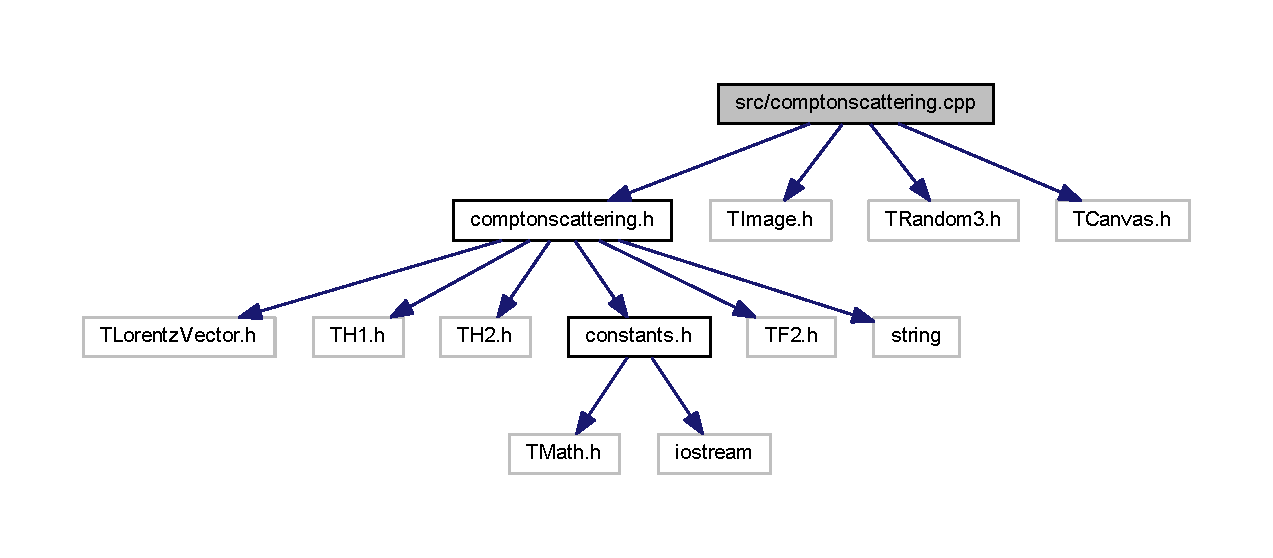
\includegraphics[width=350pt]{comptonscattering_8cpp__incl}
\end{center}
\end{figure}

\hypertarget{comptonscattering_8h}{}\section{src/comptonscattering.h File Reference}
\label{comptonscattering_8h}\index{src/comptonscattering.\+h@{src/comptonscattering.\+h}}
{\ttfamily \#include \char`\"{}T\+Lorentz\+Vector.\+h\char`\"{}}\\*
{\ttfamily \#include \char`\"{}T\+H1.\+h\char`\"{}}\\*
{\ttfamily \#include \char`\"{}T\+H2.\+h\char`\"{}}\\*
{\ttfamily \#include \char`\"{}constants.\+h\char`\"{}}\\*
{\ttfamily \#include \char`\"{}T\+F2.\+h\char`\"{}}\\*
{\ttfamily \#include $<$string$>$}\\*
Include dependency graph for comptonscattering.\+h\+:\nopagebreak
\begin{figure}[H]
\begin{center}
\leavevmode
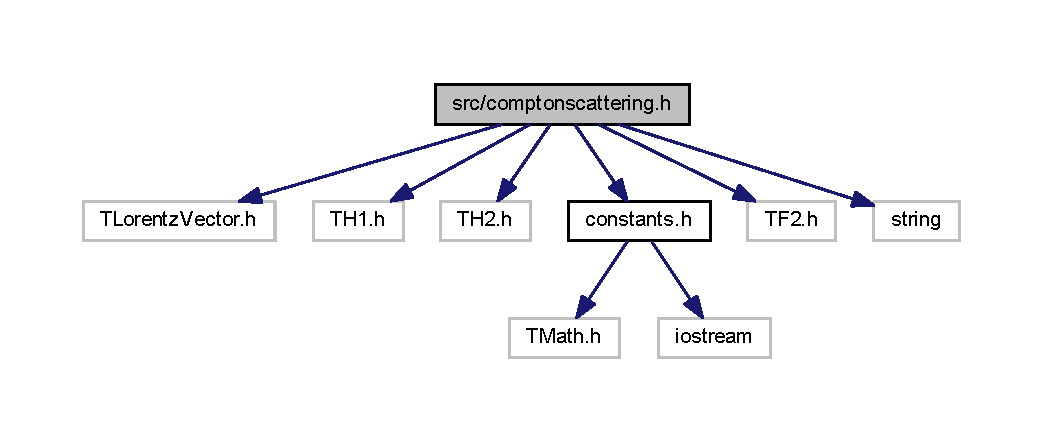
\includegraphics[width=350pt]{comptonscattering_8h__incl}
\end{center}
\end{figure}
This graph shows which files directly or indirectly include this file\+:\nopagebreak
\begin{figure}[H]
\begin{center}
\leavevmode
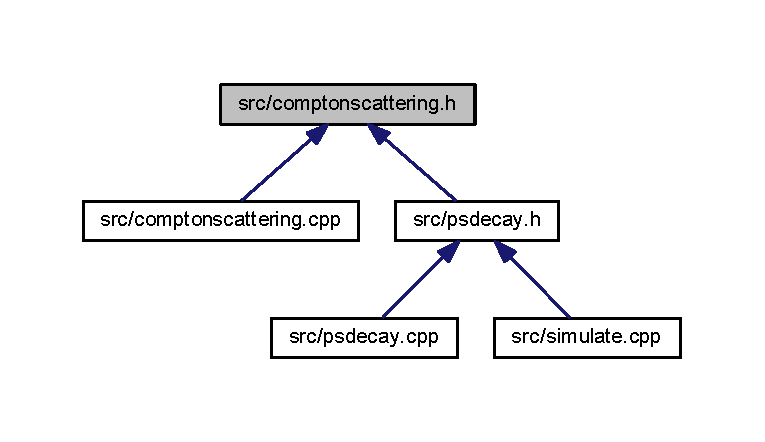
\includegraphics[width=350pt]{comptonscattering_8h__dep__incl}
\end{center}
\end{figure}
\subsection*{Classes}
\begin{DoxyCompactItemize}
\item 
class \hyperlink{classComptonScattering}{Compton\+Scattering}
\begin{DoxyCompactList}\small\item\em The \hyperlink{classComptonScattering}{Compton\+Scattering} class Class responsible for Compton scattering according to the Klein-\/\+Nishina formula. \end{DoxyCompactList}\end{DoxyCompactItemize}

\hypertarget{constants_8h}{}\section{src/constants.h File Reference}
\label{constants_8h}\index{src/constants.\+h@{src/constants.\+h}}
{\ttfamily \#include \char`\"{}T\+Math.\+h\char`\"{}}\\*
{\ttfamily \#include $<$iostream$>$}\\*
Include dependency graph for constants.\+h\+:\nopagebreak
\begin{figure}[H]
\begin{center}
\leavevmode
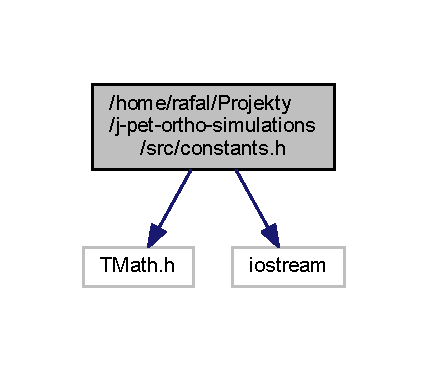
\includegraphics[width=206pt]{constants_8h__incl}
\end{center}
\end{figure}
This graph shows which files directly or indirectly include this file\+:\nopagebreak
\begin{figure}[H]
\begin{center}
\leavevmode
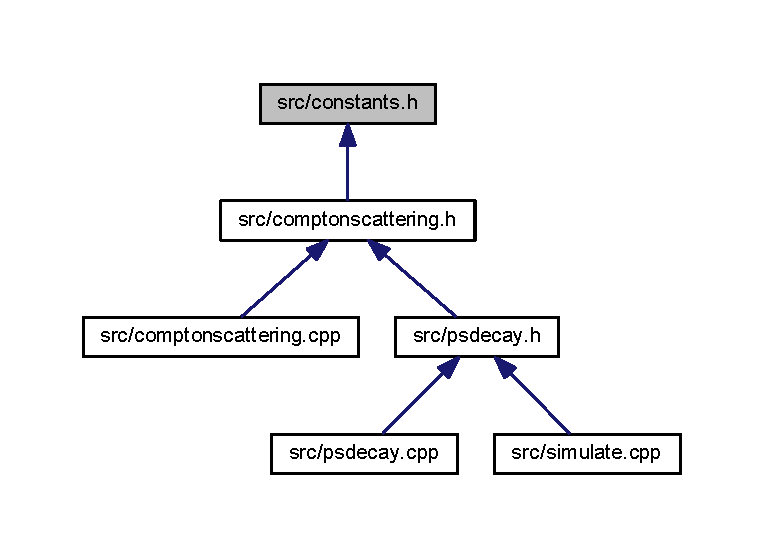
\includegraphics[width=350pt]{constants_8h__dep__incl}
\end{center}
\end{figure}
\subsection*{Functions}
\begin{DoxyCompactItemize}
\item 
void \hyperlink{constants_8h_aa8284d6930df5bb1abe506364d579b04}{Print\+Constants} ()
\begin{DoxyCompactList}\small\item\em Print\+Constants Prints to the standard output all physics constants defined in \hyperlink{constants_8h}{constants.\+h}. \end{DoxyCompactList}\end{DoxyCompactItemize}
\subsection*{Variables}
\begin{DoxyCompactItemize}
\item 
const long double \hyperlink{constants_8h_a94810453bb92e7ee5773585ae90baebe}{fine\+\_\+structure\+\_\+const\+\_\+} = 0.\+0072973525664L
\item 
const long double \hyperlink{constants_8h_af9d188b3dbc1caa192b3f37ebe5f6805}{h\+\_\+bar\+\_\+\+SI} = 1.\+054571800\+L$\ast$\+T\+Math\+::\+Power(10, -\/34)
\item 
const long double \hyperlink{constants_8h_a2ae3a758bdc777517f8c1702a8a8c738}{h\+\_\+bar\+\_\+eV} = 6.\+582119514\+L$\ast$\+T\+Math\+::\+Power(10, -\/16)
\item 
const long double \hyperlink{constants_8h_a66ce5e8f4114a5b4aa0af15cff2062b4}{light\+\_\+speed\+\_\+\+SI} = 299792458L
\item 
const long double \hyperlink{constants_8h_ae5157e847174549da78244ab23b7086a}{e\+\_\+mass\+\_\+\+SI} = 9.\+10938356\+L $\ast$ T\+Math\+::\+Power(10, -\/31)
\item 
const long double \hyperlink{constants_8h_a358559558d49e75ad6ace507cb0cd27f}{e\+\_\+mass\+\_\+\+MeV} = 0.\+5109989461L
\item 
const long double \hyperlink{constants_8h_a420beade9f7f09451ca604825847ca04}{r\+\_\+\+Compton\+\_\+\+SI} = \hyperlink{constants_8h_a2ae3a758bdc777517f8c1702a8a8c738}{h\+\_\+bar\+\_\+eV}$\ast$\hyperlink{constants_8h_a66ce5e8f4114a5b4aa0af15cff2062b4}{light\+\_\+speed\+\_\+\+SI}/(\hyperlink{constants_8h_a358559558d49e75ad6ace507cb0cd27f}{e\+\_\+mass\+\_\+\+MeV}$\ast$1000000)
\end{DoxyCompactItemize}


\subsection{Function Documentation}
\index{constants.\+h@{constants.\+h}!Print\+Constants@{Print\+Constants}}
\index{Print\+Constants@{Print\+Constants}!constants.\+h@{constants.\+h}}
\subsubsection[{\texorpdfstring{Print\+Constants()}{PrintConstants()}}]{\setlength{\rightskip}{0pt plus 5cm}void Print\+Constants (
\begin{DoxyParamCaption}
{}
\end{DoxyParamCaption}
)\hspace{0.3cm}{\ttfamily [inline]}}\hypertarget{constants_8h_aa8284d6930df5bb1abe506364d579b04}{}\label{constants_8h_aa8284d6930df5bb1abe506364d579b04}


Print\+Constants Prints to the standard output all physics constants defined in \hyperlink{constants_8h}{constants.\+h}. 



\subsection{Variable Documentation}
\index{constants.\+h@{constants.\+h}!e\+\_\+mass\+\_\+\+MeV@{e\+\_\+mass\+\_\+\+MeV}}
\index{e\+\_\+mass\+\_\+\+MeV@{e\+\_\+mass\+\_\+\+MeV}!constants.\+h@{constants.\+h}}
\subsubsection[{\texorpdfstring{e\+\_\+mass\+\_\+\+MeV}{e_mass_MeV}}]{\setlength{\rightskip}{0pt plus 5cm}const long double e\+\_\+mass\+\_\+\+MeV = 0.\+5109989461L}\hypertarget{constants_8h_a358559558d49e75ad6ace507cb0cd27f}{}\label{constants_8h_a358559558d49e75ad6ace507cb0cd27f}
\index{constants.\+h@{constants.\+h}!e\+\_\+mass\+\_\+\+SI@{e\+\_\+mass\+\_\+\+SI}}
\index{e\+\_\+mass\+\_\+\+SI@{e\+\_\+mass\+\_\+\+SI}!constants.\+h@{constants.\+h}}
\subsubsection[{\texorpdfstring{e\+\_\+mass\+\_\+\+SI}{e_mass_SI}}]{\setlength{\rightskip}{0pt plus 5cm}const long double e\+\_\+mass\+\_\+\+SI = 9.\+10938356\+L $\ast$ T\+Math\+::\+Power(10, -\/31)}\hypertarget{constants_8h_ae5157e847174549da78244ab23b7086a}{}\label{constants_8h_ae5157e847174549da78244ab23b7086a}
\index{constants.\+h@{constants.\+h}!fine\+\_\+structure\+\_\+const\+\_\+@{fine\+\_\+structure\+\_\+const\+\_\+}}
\index{fine\+\_\+structure\+\_\+const\+\_\+@{fine\+\_\+structure\+\_\+const\+\_\+}!constants.\+h@{constants.\+h}}
\subsubsection[{\texorpdfstring{fine\+\_\+structure\+\_\+const\+\_\+}{fine_structure_const_}}]{\setlength{\rightskip}{0pt plus 5cm}const long double fine\+\_\+structure\+\_\+const\+\_\+ = 0.\+0072973525664L}\hypertarget{constants_8h_a94810453bb92e7ee5773585ae90baebe}{}\label{constants_8h_a94810453bb92e7ee5773585ae90baebe}
\index{constants.\+h@{constants.\+h}!h\+\_\+bar\+\_\+eV@{h\+\_\+bar\+\_\+eV}}
\index{h\+\_\+bar\+\_\+eV@{h\+\_\+bar\+\_\+eV}!constants.\+h@{constants.\+h}}
\subsubsection[{\texorpdfstring{h\+\_\+bar\+\_\+eV}{h_bar_eV}}]{\setlength{\rightskip}{0pt plus 5cm}const long double h\+\_\+bar\+\_\+eV = 6.\+582119514\+L$\ast$\+T\+Math\+::\+Power(10, -\/16)}\hypertarget{constants_8h_a2ae3a758bdc777517f8c1702a8a8c738}{}\label{constants_8h_a2ae3a758bdc777517f8c1702a8a8c738}
\index{constants.\+h@{constants.\+h}!h\+\_\+bar\+\_\+\+SI@{h\+\_\+bar\+\_\+\+SI}}
\index{h\+\_\+bar\+\_\+\+SI@{h\+\_\+bar\+\_\+\+SI}!constants.\+h@{constants.\+h}}
\subsubsection[{\texorpdfstring{h\+\_\+bar\+\_\+\+SI}{h_bar_SI}}]{\setlength{\rightskip}{0pt plus 5cm}const long double h\+\_\+bar\+\_\+\+SI = 1.\+054571800\+L$\ast$\+T\+Math\+::\+Power(10, -\/34)}\hypertarget{constants_8h_af9d188b3dbc1caa192b3f37ebe5f6805}{}\label{constants_8h_af9d188b3dbc1caa192b3f37ebe5f6805}
\index{constants.\+h@{constants.\+h}!light\+\_\+speed\+\_\+\+SI@{light\+\_\+speed\+\_\+\+SI}}
\index{light\+\_\+speed\+\_\+\+SI@{light\+\_\+speed\+\_\+\+SI}!constants.\+h@{constants.\+h}}
\subsubsection[{\texorpdfstring{light\+\_\+speed\+\_\+\+SI}{light_speed_SI}}]{\setlength{\rightskip}{0pt plus 5cm}const long double light\+\_\+speed\+\_\+\+SI = 299792458L}\hypertarget{constants_8h_a66ce5e8f4114a5b4aa0af15cff2062b4}{}\label{constants_8h_a66ce5e8f4114a5b4aa0af15cff2062b4}
\index{constants.\+h@{constants.\+h}!r\+\_\+\+Compton\+\_\+\+SI@{r\+\_\+\+Compton\+\_\+\+SI}}
\index{r\+\_\+\+Compton\+\_\+\+SI@{r\+\_\+\+Compton\+\_\+\+SI}!constants.\+h@{constants.\+h}}
\subsubsection[{\texorpdfstring{r\+\_\+\+Compton\+\_\+\+SI}{r_Compton_SI}}]{\setlength{\rightskip}{0pt plus 5cm}const long double r\+\_\+\+Compton\+\_\+\+SI = {\bf h\+\_\+bar\+\_\+eV}$\ast${\bf light\+\_\+speed\+\_\+\+SI}/({\bf e\+\_\+mass\+\_\+\+MeV}$\ast$1000000)}\hypertarget{constants_8h_a420beade9f7f09451ca604825847ca04}{}\label{constants_8h_a420beade9f7f09451ca604825847ca04}

\hypertarget{parammanager_8cpp}{}\section{/home/rafal/\+Projekty/j-\/pet-\/ortho-\/simulations/src/parammanager.cpp File Reference}
\label{parammanager_8cpp}\index{/home/rafal/\+Projekty/j-\/pet-\/ortho-\/simulations/src/parammanager.\+cpp@{/home/rafal/\+Projekty/j-\/pet-\/ortho-\/simulations/src/parammanager.\+cpp}}
{\ttfamily \#include \char`\"{}parammanager.\+h\char`\"{}}\\*
{\ttfamily \#include $<$iostream$>$}\\*
{\ttfamily \#include $<$sstream$>$}\\*
{\ttfamily \#include $<$fstream$>$}\\*
{\ttfamily \#include $<$typeinfo$>$}\\*
{\ttfamily \#include $<$iterator$>$}\\*
Include dependency graph for parammanager.\+cpp\+:
\nopagebreak
\begin{figure}[H]
\begin{center}
\leavevmode
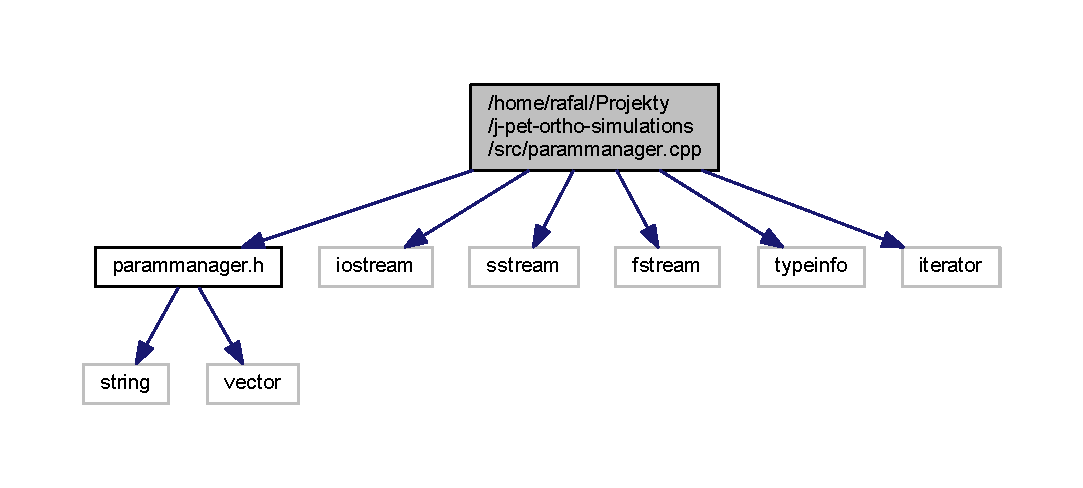
\includegraphics[width=350pt]{parammanager_8cpp__incl}
\end{center}
\end{figure}

\hypertarget{parammanager_8h}{}\section{src/parammanager.h File Reference}
\label{parammanager_8h}\index{src/parammanager.\+h@{src/parammanager.\+h}}
{\ttfamily \#include $<$string$>$}\\*
{\ttfamily \#include $<$vector$>$}\\*
Include dependency graph for parammanager.\+h\+:
\nopagebreak
\begin{figure}[H]
\begin{center}
\leavevmode
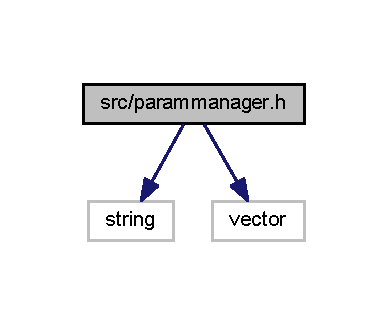
\includegraphics[width=186pt]{parammanager_8h__incl}
\end{center}
\end{figure}
This graph shows which files directly or indirectly include this file\+:
\nopagebreak
\begin{figure}[H]
\begin{center}
\leavevmode
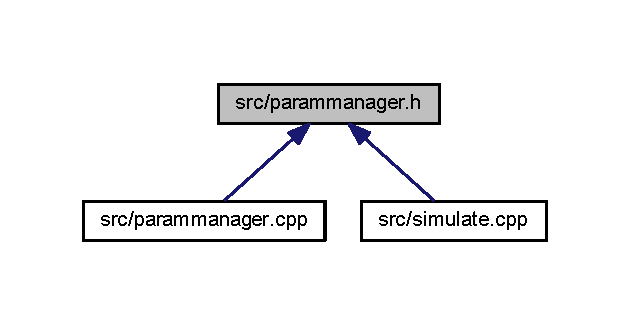
\includegraphics[width=303pt]{parammanager_8h__dep__incl}
\end{center}
\end{figure}
\subsection*{Classes}
\begin{DoxyCompactItemize}
\item 
class \hyperlink{classParamManager}{Param\+Manager}
\begin{DoxyCompactList}\small\item\em The \hyperlink{classParamManager}{Param\+Manager} class Class responsible for loadind simulation parameters from external file. (by default simulation\+\_\+parameters.\+par) \end{DoxyCompactList}\end{DoxyCompactItemize}

\hypertarget{psdecay_8cpp}{}\section{/home/rafal/\+Projekty/j-\/pet-\/ortho-\/simulations/src/psdecay.cpp File Reference}
\label{psdecay_8cpp}\index{/home/rafal/\+Projekty/j-\/pet-\/ortho-\/simulations/src/psdecay.\+cpp@{/home/rafal/\+Projekty/j-\/pet-\/ortho-\/simulations/src/psdecay.\+cpp}}
{\ttfamily \#include \char`\"{}psdecay.\+h\char`\"{}}\\*
{\ttfamily \#include $<$typeinfo$>$}\\*
{\ttfamily \#include $<$cstdio$>$}\\*
{\ttfamily \#include \char`\"{}T\+Text.\+h\char`\"{}}\\*
{\ttfamily \#include $<$iomanip$>$}\\*
{\ttfamily \#include \char`\"{}T\+Random3.\+h\char`\"{}}\\*
Include dependency graph for psdecay.\+cpp\+:
\nopagebreak
\begin{figure}[H]
\begin{center}
\leavevmode
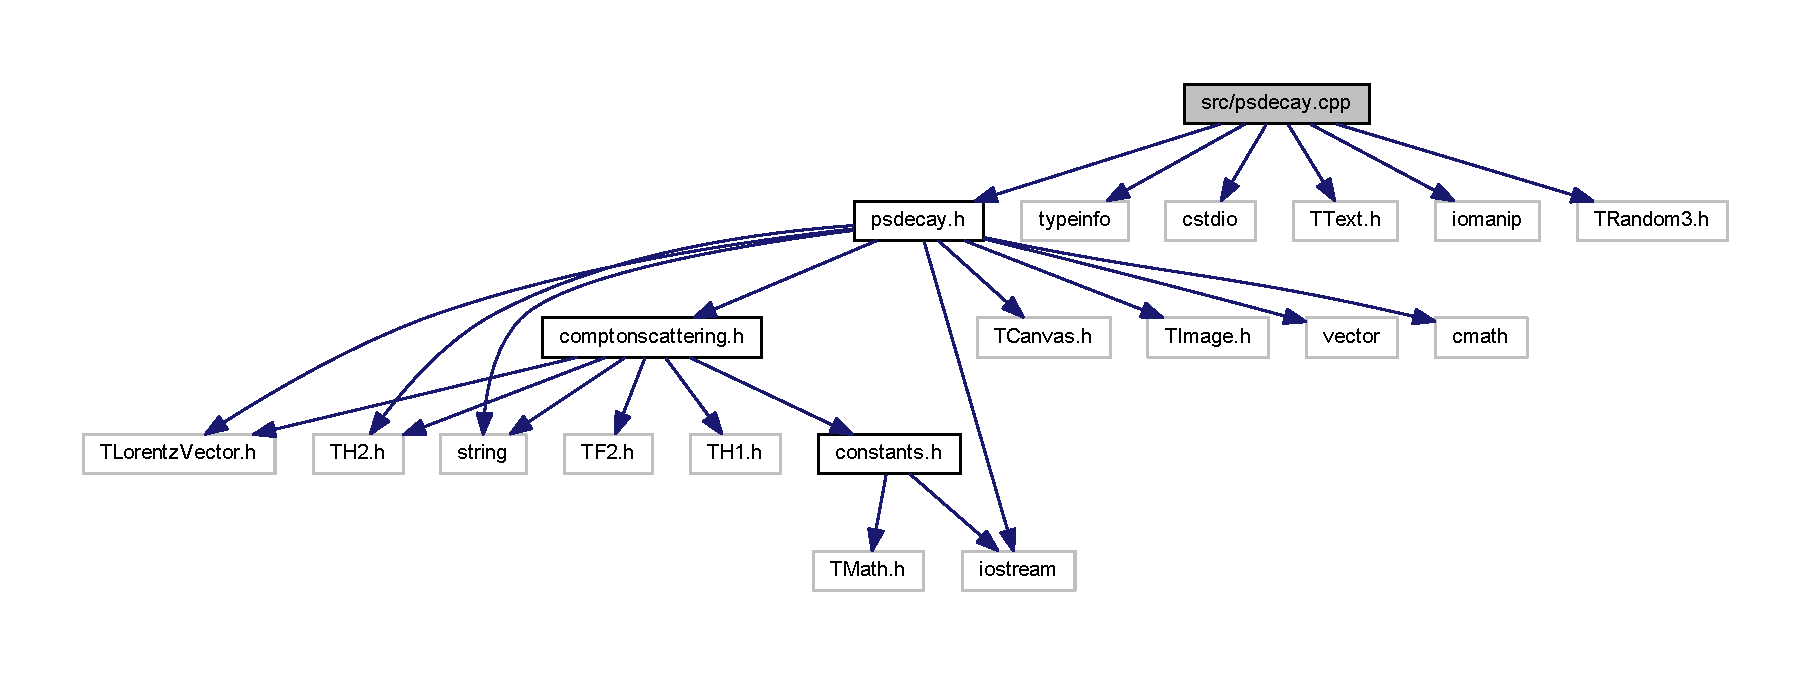
\includegraphics[width=350pt]{psdecay_8cpp__incl}
\end{center}
\end{figure}

\hypertarget{psdecay_8h}{}\section{src/psdecay.h File Reference}
\label{psdecay_8h}\index{src/psdecay.\+h@{src/psdecay.\+h}}
{\ttfamily \#include \char`\"{}T\+Lorentz\+Vector.\+h\char`\"{}}\\*
{\ttfamily \#include \char`\"{}T\+H2.\+h\char`\"{}}\\*
{\ttfamily \#include \char`\"{}T\+Canvas.\+h\char`\"{}}\\*
{\ttfamily \#include \char`\"{}T\+Image.\+h\char`\"{}}\\*
{\ttfamily \#include $<$vector$>$}\\*
{\ttfamily \#include $<$iostream$>$}\\*
{\ttfamily \#include $<$string$>$}\\*
{\ttfamily \#include $<$cmath$>$}\\*
{\ttfamily \#include \char`\"{}comptonscattering.\+h\char`\"{}}\\*
Include dependency graph for psdecay.\+h\+:\nopagebreak
\begin{figure}[H]
\begin{center}
\leavevmode
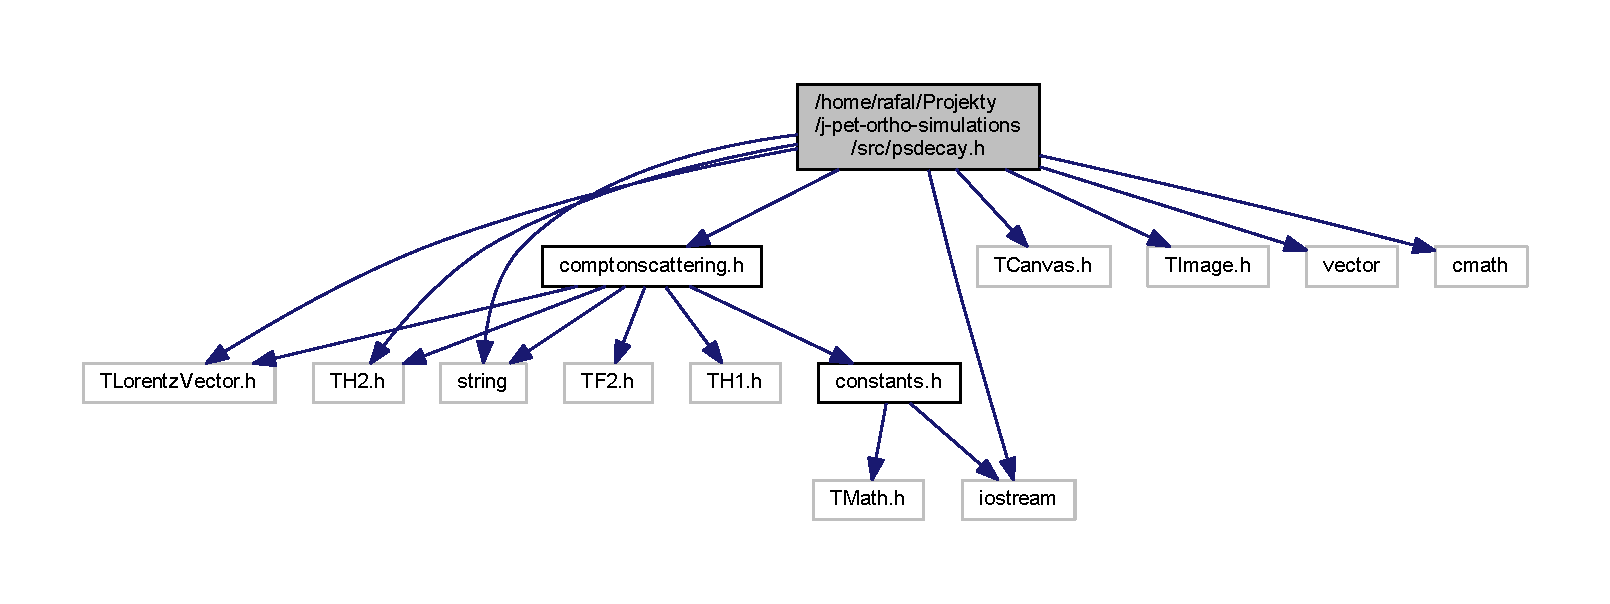
\includegraphics[width=350pt]{psdecay_8h__incl}
\end{center}
\end{figure}
This graph shows which files directly or indirectly include this file\+:\nopagebreak
\begin{figure}[H]
\begin{center}
\leavevmode
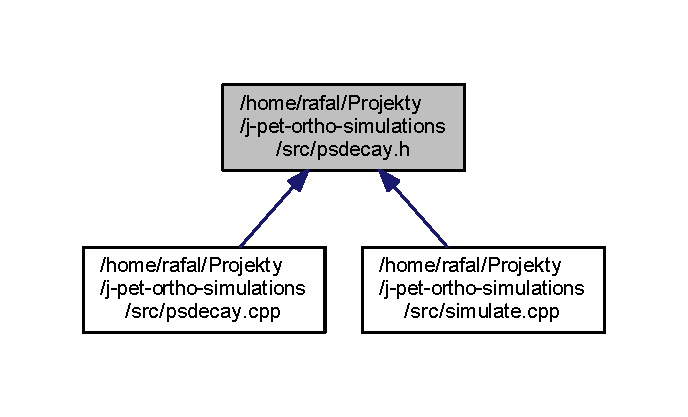
\includegraphics[width=276pt]{psdecay_8h__dep__incl}
\end{center}
\end{figure}
\subsection*{Classes}
\begin{DoxyCompactItemize}
\item 
class \hyperlink{classPsDecay}{Ps\+Decay}
\begin{DoxyCompactList}\small\item\em The \hyperlink{classPsDecay}{Ps\+Decay} class Contains histograms with gammas\textquotesingle{} characteristics and inforamtion about passed cuts.. \end{DoxyCompactList}\end{DoxyCompactItemize}


\subsection{Detailed Description}
\begin{DoxyAuthor}{Author}
Rafal Maselek \href{mailto:rafal.maselek@ncbj.gov.pl}{\tt rafal.\+maselek@ncbj.\+gov.\+pl} 
\end{DoxyAuthor}
\begin{DoxyDate}{Date}
01.\+06.\+2017 
\end{DoxyDate}

\hypertarget{simulate_8cpp}{}\section{src/simulate.cpp File Reference}
\label{simulate_8cpp}\index{src/simulate.\+cpp@{src/simulate.\+cpp}}
{\ttfamily \#include \char`\"{}psdecay.\+h\char`\"{}}\\*
{\ttfamily \#include \char`\"{}T\+Gen\+Phase\+Space.\+h\char`\"{}}\\*
{\ttfamily \#include $<$iomanip$>$}\\*
{\ttfamily \#include \char`\"{}parammanager.\+h\char`\"{}}\\*
{\ttfamily \#include $<$sys/stat.\+h$>$}\\*
{\ttfamily \#include $<$sstream$>$}\\*
Include dependency graph for simulate.\+cpp\+:\nopagebreak
\begin{figure}[H]
\begin{center}
\leavevmode
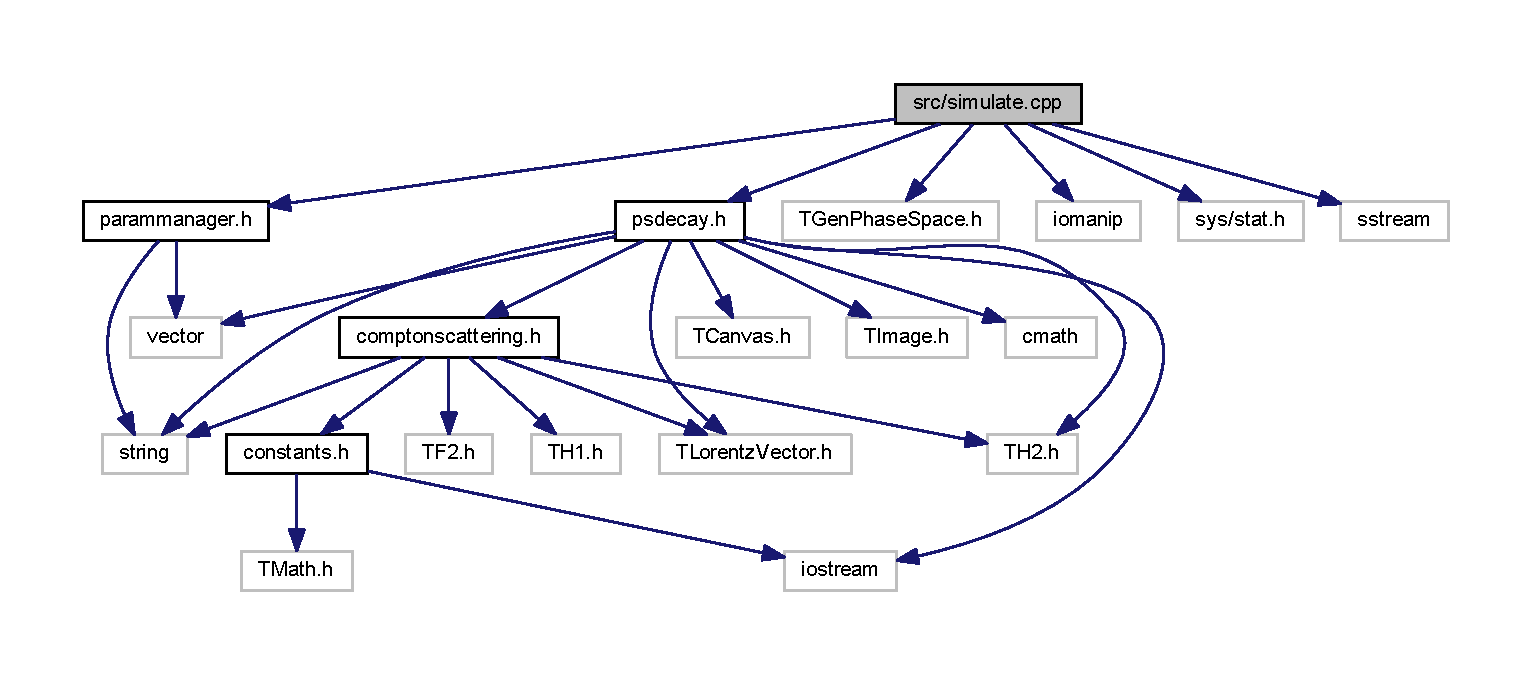
\includegraphics[width=350pt]{simulate_8cpp__incl}
\end{center}
\end{figure}
\subsection*{Functions}
\begin{DoxyCompactItemize}
\item 
static std\+::string \hyperlink{simulate_8cpp_a444f28cefb24d90ebbc3d304698f4ae6}{general\+Prefix} (\char`\"{}results/\char`\"{})
\item 
{\footnotesize template$<$typename T $>$ }\\std\+::string \hyperlink{simulate_8cpp_a6baf1eea32bd2e429a23a0f147c573b9}{to\+\_\+string} (const T a\+\_\+value)
\begin{DoxyCompactList}\small\item\em Template used to cast any value to string. Mainly used to cast double to string, preserving scientific notation. \end{DoxyCompactList}\item 
\hyperlink{classPsDecay}{Ps\+Decay} $\ast$ \hyperlink{simulate_8cpp_aa7b0b81d052171427ae22e0e350acea6}{simulate\+Decay} (T\+Lorentz\+Vector Ps, const int no\+Of\+Gammas, std\+::string file\+Prefix, int sim\+Steps=1000, double $\ast$source\+X\+YZ=nullptr)
\begin{DoxyCompactList}\small\item\em simulate\+Decay Runs Ps-\/$>$2 or Ps-\/$>$3 gamma decay. \end{DoxyCompactList}\item 
void \hyperlink{simulate_8cpp_af00dd037aec8987144d17b43882ce4c7}{simulate} (int sim\+Run, int no\+Of\+Gammas=0, \hyperlink{classParamManager}{Param\+Manager} $\ast$p\+Manag=nullptr)
\begin{DoxyCompactList}\small\item\em simulate Main function of the simulation. \end{DoxyCompactList}\item 
int \hyperlink{simulate_8cpp_a0ddf1224851353fc92bfbff6f499fa97}{main} (int argc, char $\ast$argv\mbox{[}$\,$\mbox{]})
\begin{DoxyCompactList}\small\item\em main C++ wrapper of simulate function. \end{DoxyCompactList}\end{DoxyCompactItemize}
\subsection*{Variables}
\begin{DoxyCompactItemize}
\item 
static std\+::string \hyperlink{simulate_8cpp_a3772e236af097985dda6af9562e1a912}{compton\+Prefix} = \hyperlink{simulate_8cpp_a444f28cefb24d90ebbc3d304698f4ae6}{general\+Prefix} + std\+::string(\char`\"{}compton/\char`\"{})
\item 
static std\+::string \hyperlink{simulate_8cpp_ac608ac1c2715f9bc43a256abed7ca7ee}{decays\+Prefix} = \hyperlink{simulate_8cpp_a444f28cefb24d90ebbc3d304698f4ae6}{general\+Prefix} + std\+::string(\char`\"{}decays/\char`\"{})
\end{DoxyCompactItemize}


\subsection{Detailed Description}
\begin{DoxyAuthor}{Author}
Rafal Maselek \href{mailto:rafal.maselek@ncbj.gov.pl}{\tt rafal.\+maselek@ncbj.\+gov.\+pl} 
\end{DoxyAuthor}
\begin{DoxyDate}{Date}
14.\+06.\+2017 
\end{DoxyDate}
\begin{DoxyVersion}{Version}
1.\+2
\end{DoxyVersion}
\hypertarget{simulate_8cpp_DESCRIPTION}{}\subsection{D\+E\+S\+C\+R\+I\+P\+T\+I\+ON}\label{simulate_8cpp_DESCRIPTION}
Simple simulation of positronium decay to 2 or 3 gammas.\hypertarget{simulate_8cpp_USAGE}{}\subsection{U\+S\+A\+GE}\label{simulate_8cpp_USAGE}
To use, compile using Makefile, then run. Passing 2 or 3 as argument you specify the type of decay to be generated. If another or no argument is specified, both scenarios will be generated. 

\subsection{Function Documentation}
\index{simulate.\+cpp@{simulate.\+cpp}!general\+Prefix@{general\+Prefix}}
\index{general\+Prefix@{general\+Prefix}!simulate.\+cpp@{simulate.\+cpp}}
\subsubsection[{\texorpdfstring{general\+Prefix(""results/"")}{generalPrefix("results/")}}]{\setlength{\rightskip}{0pt plus 5cm}static std\+::string general\+Prefix (
\begin{DoxyParamCaption}
\item[{\char`\"{}results/\char`\"{}}]{}
\end{DoxyParamCaption}
)\hspace{0.3cm}{\ttfamily [static]}}\hypertarget{simulate_8cpp_a444f28cefb24d90ebbc3d304698f4ae6}{}\label{simulate_8cpp_a444f28cefb24d90ebbc3d304698f4ae6}
\index{simulate.\+cpp@{simulate.\+cpp}!main@{main}}
\index{main@{main}!simulate.\+cpp@{simulate.\+cpp}}
\subsubsection[{\texorpdfstring{main(int argc, char $\ast$argv[])}{main(int argc, char *argv[])}}]{\setlength{\rightskip}{0pt plus 5cm}int main (
\begin{DoxyParamCaption}
\item[{int}]{argc, }
\item[{char $\ast$}]{argv\mbox{[}$\,$\mbox{]}}
\end{DoxyParamCaption}
)}\hypertarget{simulate_8cpp_a0ddf1224851353fc92bfbff6f499fa97}{}\label{simulate_8cpp_a0ddf1224851353fc92bfbff6f499fa97}


main C++ wrapper of simulate function. 


\begin{DoxyParams}{Parameters}
{\em argc} & Number of provided arguments. \\
\hline
{\em argv} & Array of arguments. \\
\hline
\end{DoxyParams}
\begin{DoxyReturn}{Returns}
0 
\end{DoxyReturn}
\index{simulate.\+cpp@{simulate.\+cpp}!simulate@{simulate}}
\index{simulate@{simulate}!simulate.\+cpp@{simulate.\+cpp}}
\subsubsection[{\texorpdfstring{simulate(int sim\+Run, int no\+Of\+Gammas=0, Param\+Manager $\ast$p\+Manag=nullptr)}{simulate(int simRun, int noOfGammas=0, ParamManager *pManag=nullptr)}}]{\setlength{\rightskip}{0pt plus 5cm}void simulate (
\begin{DoxyParamCaption}
\item[{int}]{sim\+Run, }
\item[{int}]{no\+Of\+Gammas = {\ttfamily 0}, }
\item[{{\bf Param\+Manager} $\ast$}]{p\+Manag = {\ttfamily nullptr}}
\end{DoxyParamCaption}
)}\hypertarget{simulate_8cpp_af00dd037aec8987144d17b43882ce4c7}{}\label{simulate_8cpp_af00dd037aec8987144d17b43882ce4c7}


simulate Main function of the simulation. 


\begin{DoxyParams}{Parameters}
{\em sim\+Run} & Index of the run. \\
\hline
{\em no\+Of\+Gammas} & How many decay products should be simulated. If different from 2 or 3 then both scenarios are simulated. \\
\hline
{\em p\+Manag} & \hyperlink{classParamManager}{Param\+Manager} object containing parameters of the simulation and source coordinates. \\
\hline
\end{DoxyParams}
\index{simulate.\+cpp@{simulate.\+cpp}!simulate\+Decay@{simulate\+Decay}}
\index{simulate\+Decay@{simulate\+Decay}!simulate.\+cpp@{simulate.\+cpp}}
\subsubsection[{\texorpdfstring{simulate\+Decay(\+T\+Lorentz\+Vector Ps, const int no\+Of\+Gammas, std\+::string file\+Prefix, int sim\+Steps=1000, double $\ast$source\+X\+Y\+Z=nullptr)}{simulateDecay(TLorentzVector Ps, const int noOfGammas, std::string filePrefix, int simSteps=1000, double *sourceXYZ=nullptr)}}]{\setlength{\rightskip}{0pt plus 5cm}{\bf Ps\+Decay}$\ast$ simulate\+Decay (
\begin{DoxyParamCaption}
\item[{T\+Lorentz\+Vector}]{Ps, }
\item[{const int}]{no\+Of\+Gammas, }
\item[{std\+::string}]{file\+Prefix, }
\item[{int}]{sim\+Steps = {\ttfamily 1000}, }
\item[{double $\ast$}]{source\+X\+YZ = {\ttfamily nullptr}}
\end{DoxyParamCaption}
)}\hypertarget{simulate_8cpp_aa7b0b81d052171427ae22e0e350acea6}{}\label{simulate_8cpp_aa7b0b81d052171427ae22e0e350acea6}


simulate\+Decay Runs Ps-\/$>$2 or Ps-\/$>$3 gamma decay. 


\begin{DoxyParams}{Parameters}
{\em Ps} & Four vector of positronium. \textbackslash{}param no\+Of\+Gammas How many gammas are produced in a Ps decay. \\
\hline
{\em sim\+Steps} & Number of events to be simulated, also the number of simulation steps. \\
\hline
{\em source\+X\+YZ} & Three element array containg position of the source (x,y,z). \\
\hline
\end{DoxyParams}
\begin{DoxyReturn}{Returns}
An instance of \hyperlink{classPsDecay}{Ps\+Decay} class. 
\end{DoxyReturn}
\index{simulate.\+cpp@{simulate.\+cpp}!to\+\_\+string@{to\+\_\+string}}
\index{to\+\_\+string@{to\+\_\+string}!simulate.\+cpp@{simulate.\+cpp}}
\subsubsection[{\texorpdfstring{to\+\_\+string(const T a\+\_\+value)}{to_string(const T a_value)}}]{\setlength{\rightskip}{0pt plus 5cm}template$<$typename T $>$ std\+::string to\+\_\+string (
\begin{DoxyParamCaption}
\item[{const T}]{a\+\_\+value}
\end{DoxyParamCaption}
)}\hypertarget{simulate_8cpp_a6baf1eea32bd2e429a23a0f147c573b9}{}\label{simulate_8cpp_a6baf1eea32bd2e429a23a0f147c573b9}


Template used to cast any value to string. Mainly used to cast double to string, preserving scientific notation. 



\subsection{Variable Documentation}
\index{simulate.\+cpp@{simulate.\+cpp}!compton\+Prefix@{compton\+Prefix}}
\index{compton\+Prefix@{compton\+Prefix}!simulate.\+cpp@{simulate.\+cpp}}
\subsubsection[{\texorpdfstring{compton\+Prefix}{comptonPrefix}}]{\setlength{\rightskip}{0pt plus 5cm}std\+::string compton\+Prefix = {\bf general\+Prefix} + std\+::string(\char`\"{}compton/\char`\"{})\hspace{0.3cm}{\ttfamily [static]}}\hypertarget{simulate_8cpp_a3772e236af097985dda6af9562e1a912}{}\label{simulate_8cpp_a3772e236af097985dda6af9562e1a912}
\index{simulate.\+cpp@{simulate.\+cpp}!decays\+Prefix@{decays\+Prefix}}
\index{decays\+Prefix@{decays\+Prefix}!simulate.\+cpp@{simulate.\+cpp}}
\subsubsection[{\texorpdfstring{decays\+Prefix}{decaysPrefix}}]{\setlength{\rightskip}{0pt plus 5cm}std\+::string decays\+Prefix = {\bf general\+Prefix} + std\+::string(\char`\"{}decays/\char`\"{})\hspace{0.3cm}{\ttfamily [static]}}\hypertarget{simulate_8cpp_ac608ac1c2715f9bc43a256abed7ca7ee}{}\label{simulate_8cpp_ac608ac1c2715f9bc43a256abed7ca7ee}

%--- End generated contents ---

% Index
\backmatter
\newpage
\phantomsection
\clearemptydoublepage
\addcontentsline{toc}{chapter}{Index}
\printindex

\end{document}
